\section{Thermal Model Description}

In this chapter the Geometrical Mathematical Model (GMM) and the Thermal Mathematical Model
(TMM) will be discussed and presented, in respective order. Both models have been created and
evaluated with the use of \textbf{ESATAN-TMS 2022} (Project Revision 1.445).

\subsection{Geometrical Mathematical Model}

The following section is composed, firstly, by the establishment of general assumptions,
followed by a description of material properties, and, finally, by a detailed explanation
of every modelled piece and subsystem.

\subsubsection{General assumptions}
The following general assumptions have been taken in the created models and performed simulations:

\begin{itemize}
    \item External thermal sources and environment have been considered as presented in Section 4.
    \item The initial spacecraft temperature is $25^\circ C$.
    \item The satellite y-axis (+Y face) is always pointing to Nadir.
    \item Black paint is used in the internal PCBs of the satellite.
    \item White paint is used in the lateral and bottom PCBs.
    \item All PCBs can be modeled as a paralel (in-plane) and serial (cross-plane) set of thermal reistances
    defined by the properties of the materials they are constituted of.
    \item Electrical components can be modeled as Non-Geometrical Thermal Nodes with a set conductance and
    heat dissipation.
    \item All thermal and optical properties are not functions of temperature.
\end{itemize}

Despite this, some other approximations are taken in order to heavily simplify the geometry of certain pieces,
most notably, the K-Band support and the threaded screws. Both will be discussed in further sections.

\subsubsection{Material Properties}

This subsection presents the different optical and thermal properties of the materials that have been used to
define the bulks of the thermal model of the spacecraft. Seldom are these values directly assigned to a geometry,
using instead more complex combinations of them, coupled with the use of the measured mass of components.

\begin{table}[H]
    \centering
    \begin{tabular}{lccccc}
        \toprule
        \textbf{Material} & \textbf{$\varepsilon_{IR}$} & \textbf{$\alpha_s$} & \textbf{$\rho$ [kg/m$^3$]} & \textbf{$c_p$ [J/kg$\cdot$K]} & \textbf{$k$ [W/m$\cdot$K]} \\
        \midrule
        FR-4 & 0.94 & 0.12 & 1850 & 1200 & 0.8181 \\
        Copper & x & x & 8930 & 385 & 400 \\
        Teflon (PTFE) & 0.92 & 0.046 & 2070 & 1010 & 0.27 \\
        Stainless Steel (AISI304SS) & 0.075 & 0.42 & 8000 & 500 & 15 \\
        Aluminum Alloy (Alloy 7075) & 0.21 & 0.18 & 2810 & 960 & 130 \\
        RS Rogers & x & x & 2200 & 960 & 0.2 \\
        Tin & 0.11 & 0.08 & 5765 & 250 & 62 \\
        LiPo Battery* & 0.3 & 0.5 & 2750 & 1000 & 2.5 (ip), 0.6 (cp) \\
        Phosphor Bronze & x & x & 8800 & 380 & 62 \\
        Aluminum 6063-T5 & 0.77 & 0.8 & 2700 & 900 & 209 \\
        Nylon & 0.85 & 0.12 & 1150 & 1500 & 0.53 \\
        Gallium Arsenide & 0.85 & 0.91 & 5316 & 325 & 50 \\
        ABS & 0.82 & 0.94 & 1070 & 1990 & 0.162 \\
        White Paint & 0.94 & 0.19 & x & x & x \\
        Black Coat & 0.94 & 0.96 & x & x & x \\
        \bottomrule
    \end{tabular}
    \caption{Material Properties Table. *LiPo Battery values are approximated.}
    \label{tab:material_properties}
\end{table}

\paragraph{}
In order to determine the properties that are asigned to ESATAN primitives the following
procedure is followed:
\begin{itemize}
    \item $\mathbf{IR\ emissivity\ (\varepsilon_{IR})}$: The IR emissivity is computed by 
    performing a weighted average, by projected surface, of the conjunction of pieces modeled.
    \begin{equation}
        \varepsilon_{IR}=\sum_{i}\frac{A_i\cdot\varepsilon_i}{A_T}
    \end{equation}
    Where $A_T$ denotes the sum of all projected areas.
    An ilustration of this process is provided below:
    \begin{figure}[H]
        \centering
        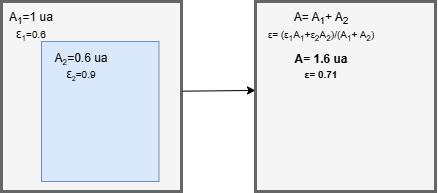
\includegraphics[width=0.5\linewidth]{res/img/5_simulationanalisys/AreasWeighted.drawio.png}
        \caption{Example or IR emissivity calculation on simplification of pieces}
        \label{fig:areaexample}
    \end{figure}
    \item $\mathbf{Solar\ Absorptivity\ (\alpha_s)}$: Solar Absorptivity is calculated following
    the same procedure as for the IR emissivity:
    \begin{equation}
        \alpha_s=\sum_{i}\frac{A_i\cdot\alpha_i}{A_T}
    \end{equation}
    \item $\mathbf{Density(\rho)}$: The density is computed by dividing the mass of the real
    component or components by the volume of the ESATAN primitive defined.
    \begin{equation}
        \rho=\frac{m_{real}}{V_{primitive}}
    \end{equation}
    \item $\mathbf{Specific\ Heat\ (c_{p})}$: The specific heat is computed as the weighted sum
    of the individual specific heats by mass of each real component:
    \begin{equation}
        c_p=\sum_i \frac{c_i \cdot m_i}{m_T}
    \end{equation}
    Where $m_T$ denotes the sum of all masses.
    \item $\mathbf{Conductivity (k)}$: The conductivity calculations will be further discussed in
    the corresponding sections of each geometry as well as in the next subsection. The approach taken is to consider different pieces
    as series or paralel resistances, computing either the weighted averaged or the harmonic mean.
    This will lead to the appearence of in-plane and crossplane conductivities, denoted as i.p. or 
    c.p. respectively.
\end{itemize}

\subsubsection{Printed Circuit Boards Conductivity and Specific Heat}
The PoCat spacecrafts make use of PCBs for the lateral boards as well as for the housing of the 
subsystems. Each one possesses a different ammount of layers and even materials, leading to variations
in conductivity. In order to simplify this problem each layer is considered a resistance, ignoring
the order of placement.
\paragraph{}
This can be visually represented as:

\begin{figure}[H]
    \centering
    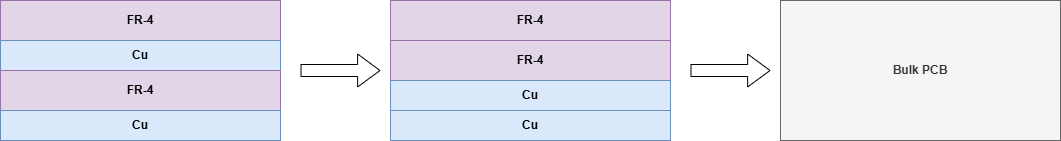
\includegraphics[width=1\linewidth]{res/img/5_simulationanalisys/resistances.png}
    \caption{Simplification of PCB layers}
    \label{fig:simpresist}
\end{figure}

Considering the amount of layers and the cumulative thickness of each type we arrive to the following
table, containing information of each one of the PCBs. Note that the antenna P/L board is also computed.

\begin{table}[H]
  \centering
  \begin{tabular}{lcccc}
      \toprule
      \textbf{PCB} & \textbf{Copper (mm)} & \textbf{FR4 (mm)} & \textbf{Mask (mm)} & \textbf{Rogers (mm)} \\
      \midrule
      OBC-COMMS            & 0.14 & 1.44 & 0.02 & 0     \\
      EPS                  & 0.14 & 1.44 & 0.02 & 0     \\
      ADCS                 & 0.14 & 1.44 & 0.02 & 0     \\
      Y+Mag                & 0.21 & 1.77 & 0.02 & 0     \\
      Laterals             & 0.21 & 1.77 & 0.02 & 0     \\
      Bottom               & 0.21 & 1.77 & 0.02 & 0     \\
      Slider               & 0.07 & 1.51 & 0.02 & 0     \\
      Kband Under          & 0.21 & 0.84 & 0.04 & 0.21  \\
      Kband Over (Antenna) & 0.14 & 1.12 & 0.04 & 0.254 \\
      \bottomrule
  \end{tabular}
  \caption{Cumulative thickness of material layers by PCB}
\end{table}
Now, in order to compute the $c_p$ as well as i.p. and c.p. conductivities we will procede with the aforementioned
methods. To calculate the conductivities we will make use of the following formulas, corresponding to the weighted and
harmonic means, respectively.
\paragraph{}
The in-plane conductivity:

\begin{equation}
    \kappa_{i.p.}=\sum_i \frac{\kappa_i \cdot l_i }{l_T}
\end{equation}

Where $\kappa_i$ denotes the in-plane conductivity of each material, $l_i$ its thickness and $l_T$ the total thickness
of the PCB.

\paragraph{}
The cross-plane conductivity:

\begin{equation}
    \kappa_{c.p.}=\left( \sum_i \frac{l_i}{\kappa_i} \right)^{-1} \cdot l_T
\end{equation}

Finally, the specific heat ($c_p$) can be computed, by imagining the PCB as an homogeneus substance, making
use of the weighted average by mass of each layer. This yields the following expression:
\begin{equation}
    c_p=\sum_i \frac{m_i \cdot c_p^i}{m_T}
\end{equation}

Due to the impossibility of measuring each layers' mass we can make use of its relation with density and volume
such that:
\begin{equation}
    m_i=V_i\cdot \rho = l_i \cdot A_i \cdot \rho_i
\end{equation}

Where $l_i$ and $A_i$ denote the length and area of the layer, respectively. Coming back to expression (7)
we finally obtain:
\begin{equation}
    c_p= \sum_i \frac{l_i \cdot A_i \cdot \rho_i \cdot c_p^i}{\sum_j l_j \cdot A_j \cdot \rho_j }
\end{equation}
As the area is equal for each layer we can extract it from the sumatory, resulting in:
\begin{equation}
    c_p= \sum_i \frac{l_i \cdot \rho_i \cdot c_p^i}{\sum_j l_j \cdot \rho_j }
\end{equation}

Using this final expression, as well as the expressions (5) and (6), with the auxilarary use of Tables 5.1
and 5.2, we compute these variables:

\begin{table}[H]
  \centering
  \begin{tabular}{lccc}
      \toprule
      \textbf{PCB} & $\mathbf{c_p\ [J/kg\cdot K]}$ & $\mathbf{k_{c.p.} [W/m\cdot K]}$ & $\mathbf{k_{i.p.} [W/m\cdot K]}$ \\
      \midrule
      OBC-COMMS            & 940  & 0.32 & 91  \\
      EPS                  & 940  & 0.32 & 91  \\
      ADCS                 & 940  & 0.32 & 91  \\
      Y+Mag                & 904  & 0.32 & 171 \\
      Laterals             & 904  & 0.32 & 171 \\
      Bottom               & 904  & 0.32 & 171 \\
      Slider               & 1050 & 0.30 & 47  \\
      Kband Under          & 783  & 0.31 & 110 \\
      Kband Over (Antenna) & 905  & 0.29 & 89  \\
      \bottomrule
  \end{tabular}
  \caption{PCB Bulk Thermal Properties}
\end{table}


\subsubsection{Introduction to the GMM}

The modelling of the spacecraft will be presented in ascending order,
grouping geometries in the same section by logical relation. As there
isn't a structure acting as the skeleton of the PocketQubes, no section
is reserved to it.
\paragraph{}
Before this, though, a general overview of the model is given .
In Figure \ref{fig:explodedview} an exploded view of PoCat-3 is presented, 
highligting some its most important components.

\begin{figure}[H]
    \centering
    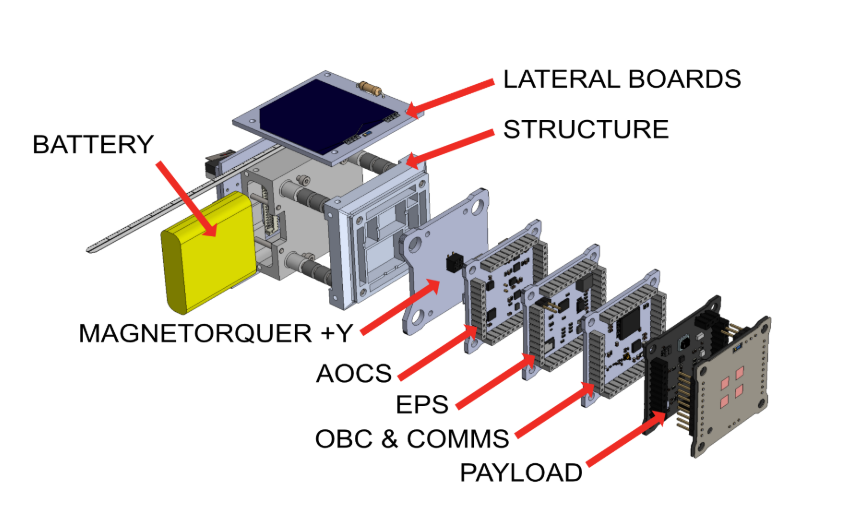
\includegraphics[width=0.6\linewidth]{res/img/5_simulationanalisys/exploded.PNG}
    \caption{Exploded view of the $^{\text{Po}}$Cat-3 spacecraft.}
    \label{fig:explodedview}
\end{figure}
Some views of the CAD model used as a reference for the creation of geometries in ESATAN
are presented next in contrast to the actual geometries modeled for the thermal analysis:

\begin{figure}[H]
    \centering
    \begin{subfigure}{.5\textwidth}
      \centering
      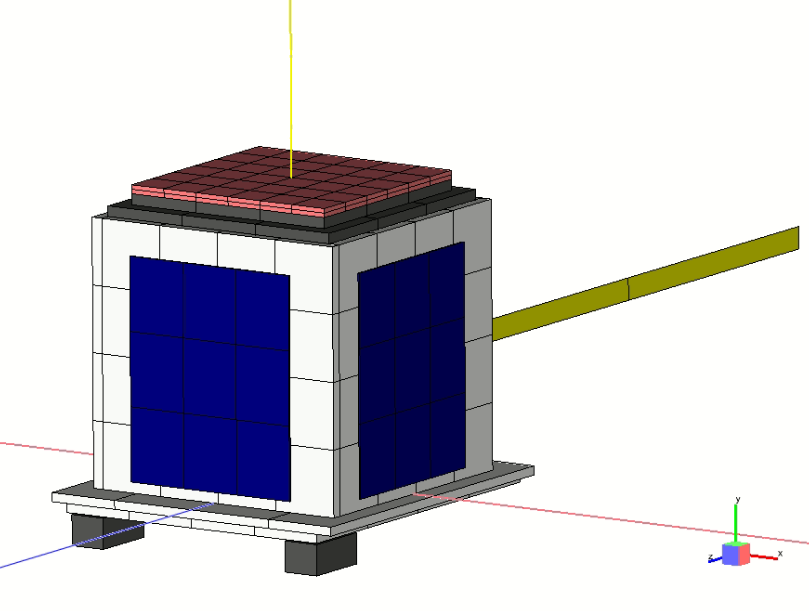
\includegraphics[width=.6\linewidth]{res/img/5_simulationanalisys/Comparisons/ESATAN/pqfull.PNG}
      \caption{PocketQube GMM in ESATAN.}
      \label{fig:pqfull}
    \end{subfigure}%
    \begin{subfigure}{.5\textwidth}
      \centering
      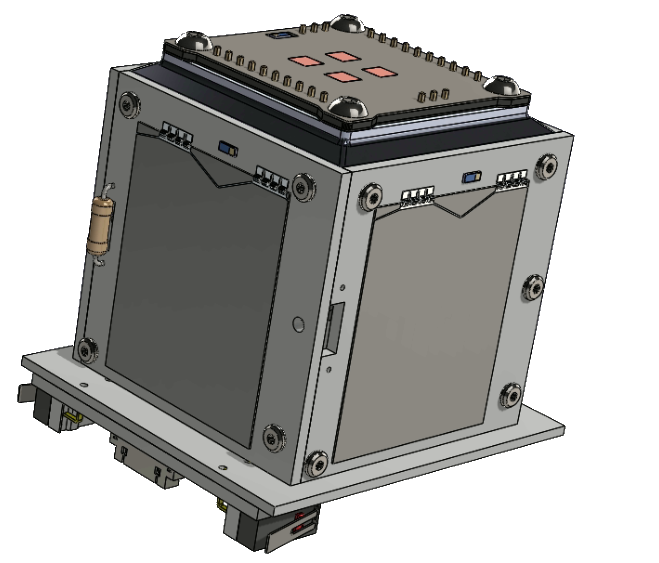
\includegraphics[width=.5\linewidth]{res/img/5_simulationanalisys/Comparisons/SLDW/pqfull_Solid.PNG}
      \caption{PocketQube CAD in Solidworks}
      \label{fig:pqfullsolid}
    \end{subfigure}
    \caption{Full GMM in ESATAN and in Solidworks.}
    \label{fig:pqfullim}
\end{figure}

Removing a lateral board in order to get a better view into the PocketQube:

\begin{figure}[H]
    \centering
    \begin{subfigure}{.5\textwidth}
      \centering
      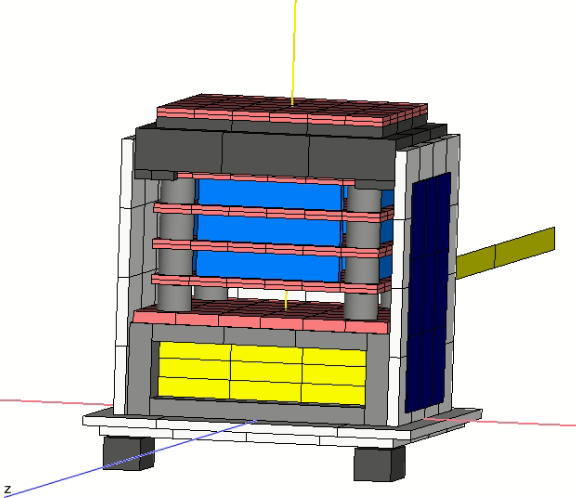
\includegraphics[width=.6\linewidth]{res/img/5_simulationanalisys/Comparisons/ESATAN/pqnolat.PNG}
      \caption{PocketQube GMM in ESATAN w/o a lateral board.}
      \label{fig:pqnolat}
    \end{subfigure}%
    \begin{subfigure}{.5\textwidth}
      \centering
      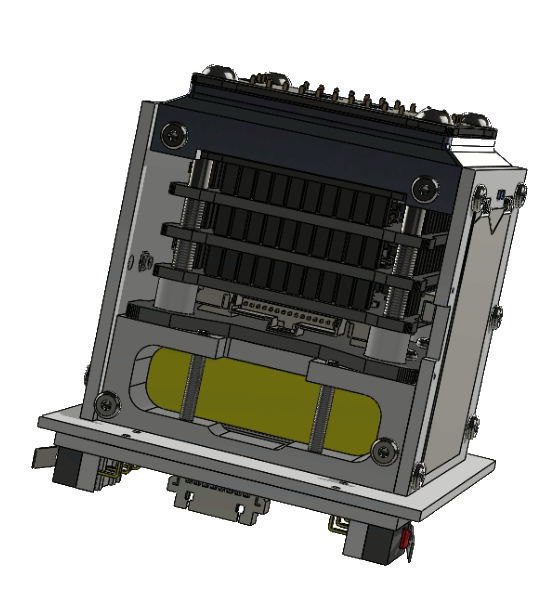
\includegraphics[width=.5\linewidth]{res/img/5_simulationanalisys/Comparisons/SLDW/pqnolat_Solid.PNG}
      \caption{PocketQube GMM in Solidworks w/o a lateral board.}
      \label{fig:pqnolatsolid}
    \end{subfigure}
    \caption{PocketQube GMM in ESATAN and Solidworks w/o a lateral board.}
    \label{fig:pqnolatim}
\end{figure}


\subsubsection{Killswitches}
The killswitches act as the interruptor enabling power of the spacecraft as it is released into
orbit. They are mainly composed by main rectangular body, where the internal circuitry is located,
covered by a black plastic case, the levers, that serve as the actuators of the interruptor, and
the legs that connect to the bottom board.

\paragraph{}

Considering the small crossection of the levers and the legs, the killswitches are geometrically
modeled as a simple solid rectangular prism. The visual representation and comparison with the CAD
is presented next: 

\begin{figure}[H]
    \centering
    \begin{subfigure}{.5\textwidth}
      \centering
      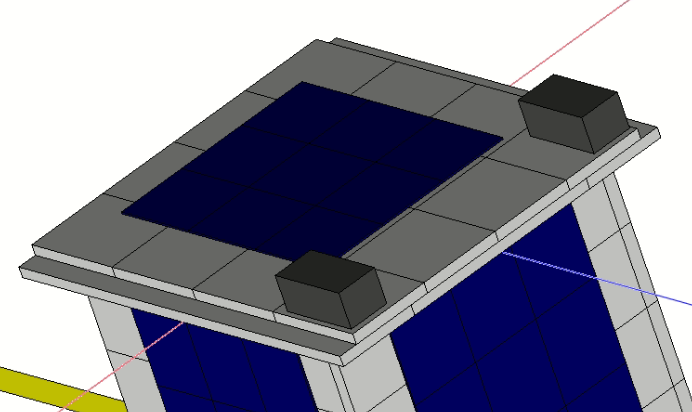
\includegraphics[width=.6\linewidth]{res/img/5_simulationanalisys/Comparisons/ESATAN/Killswitches.PNG}
      \caption{Killswitches in ESATAN (with other components)}
      \label{fig:killswitches}
    \end{subfigure}%
    \begin{subfigure}{.5\textwidth}
      \centering
      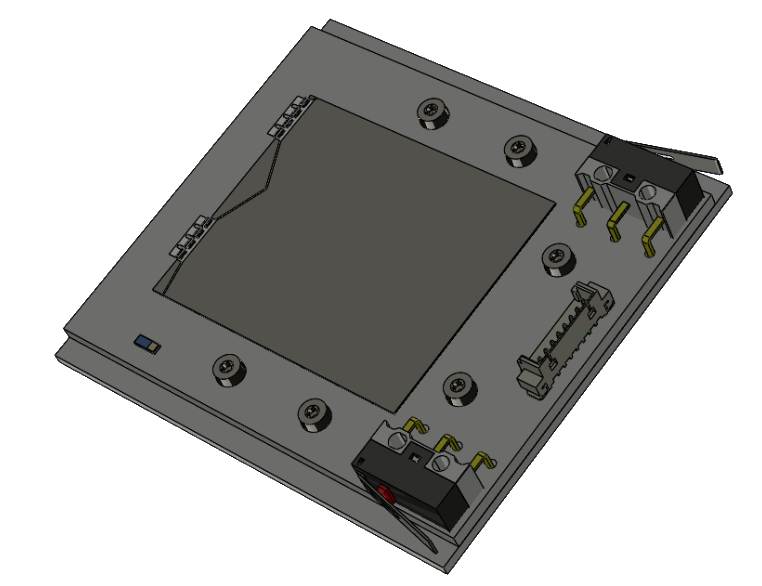
\includegraphics[width=.5\linewidth]{res/img/5_simulationanalisys/Comparisons/SLDW/BottomPCB_Solid.PNG}
      \caption{Killswitches in Solidworks (with other components)}
      \label{fig:killswitchessolid}
    \end{subfigure}
    \caption{Comparison between thermal and CAD model for the Killswitches (with other components).}
    \label{fig:killswitchesim}
\end{figure}

Providing a close-up into the killswitches:

\begin{figure}[H]
    \centering
    \begin{subfigure}{.5\textwidth}
      \centering
      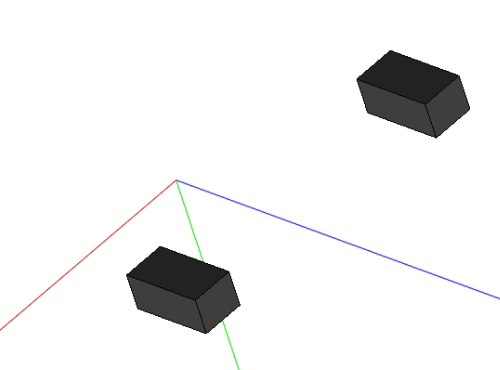
\includegraphics[width=.6\linewidth]{res/img/5_simulationanalisys/Comparisons/ESATAN/killswitches_raw.PNG}
      \caption{Killswitches in ESATAN (without other components)}
      \label{fig:killswitchesraw}
    \end{subfigure}%
    \begin{subfigure}{.5\textwidth}
      \centering
      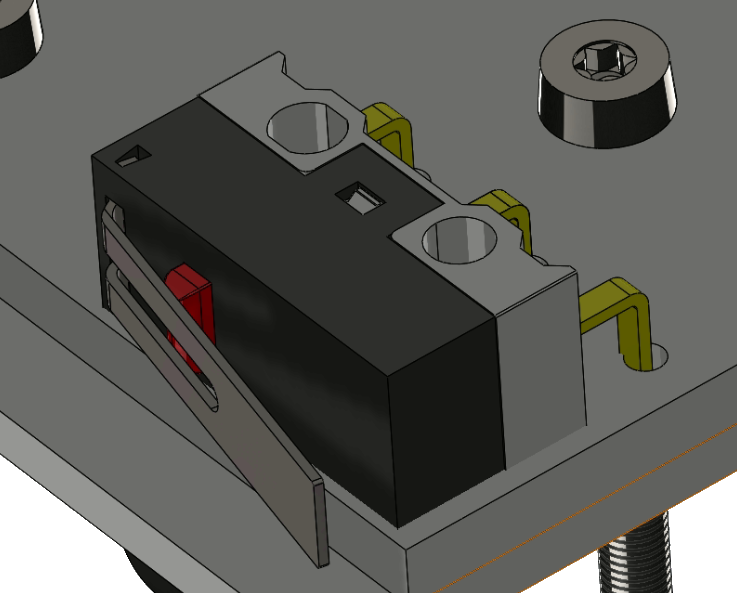
\includegraphics[width=.5\linewidth]{res/img/5_simulationanalisys/Comparisons/SLDW/Killswitch_raw_Solid.PNG}
      \caption{Killswitches in Solidworks (without other components)}
      \label{fig:killswitchesrawsolid}
    \end{subfigure}
    \caption{Comparison between thermal and CAD model for the Killswitches (witohut other components)}
    \label{fig:killswitchesrawim}
\end{figure}

The properties of the killswitches themselves, as determined by following the procedure specified in
this section are:

\begin{table}[H]
\centering
\resizebox{\columnwidth}{!}{
    \begin{tabular}{@{}cccccccccc@{}}
    \toprule
    \textbf{$SD\_KS\_PX$} & \textbf{Material} & \textbf{m (g)} & \textbf{m (kg)} & $\mathbf{m (\%)}$ & $\mathbf{V_{E}\ [m^3]}$ & $\mathbf{\rho\ [kg/m^3]}$ & $\mathbf{c_p\ [J/kg\cdot K]}$ & $\mathbf{k_{c.p.} [W/m\cdot K]}$ & $\mathbf{k_{i.p.} [W/m\cdot K]}$ \\ \midrule
    \textit{Primitive}        & ABS               & 1.2            & 0.0012          & 100                & 4.56E-07            & \textbf{2632}                     & \textbf{1990}                        & \textbf{0.162}                          & \textbf{0.162}                       \\
    {\ul Idem}            &                   &                &                 &                    &                        &                          &                             &                                &                                \\
    $SD\_KS\_NX$              & ABS               & 1.2            & 0.0012          & 100                & 4.56E-07            & \textbf{2632}                     & \textbf{1990}                        & \textbf{0.162}                          & \textbf{0.162}                   \\ \bottomrule
\end{tabular}
}
\caption{Bulk properties of the killswitches.}
\label{tab:tablapcbbulk}
\end{table}

The optical properties:

\begin{table}[H]
  \centering
  \begin{tabular}{@{}cccc@{}}
  \toprule
  \textbf{Primitive} & \textbf{Material} & $\mathbf{\epsilon_{IR}}$ & $\mathbf{\alpha_{S}}$ \\ \midrule
  SD\_KS\_PX         & ABS               & 0.82                     & 0.94                  \\ \bottomrule
  \end{tabular}
  \caption{Optical properties of the killswitches primitives.}
\end{table}

\subsubsection{Bottom Board}
The bottom board hosts some screws, a solar panel (SP-Y) and the killswitches. It is a four copper layer
PCB with a magnetorquer ingrained into it. It is made of a total of nine layers, four copper layers, three FR-4,
and two solder masks (black). 

\paragraph{}

It is modeled as a solid ortothropic rectangular prism, with the bulk properties as specified in Table \ref{tab:tablapcbbulk}
and with the optical properties of white paint as specified in Table \ref{tab:material_properties}. The components other than
the PCB itself are only considered in the calculation of density, yet ignored for the specific heat and conductivity.
The visual representation and comparison with the CAD is presented next: 

\begin{figure}[H]
    \centering
    \begin{subfigure}{.5\textwidth}
      \centering
      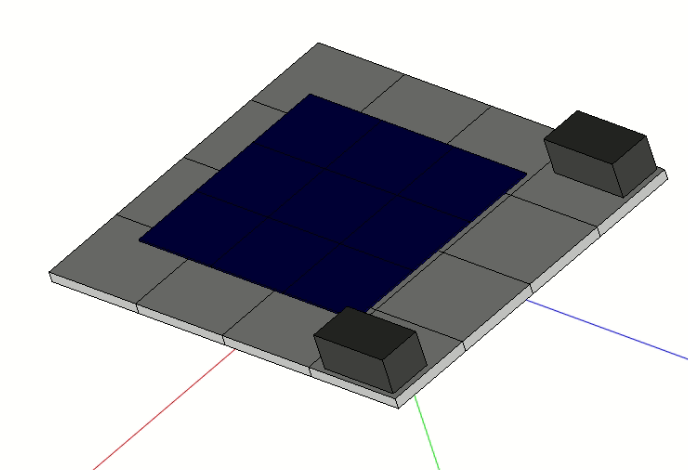
\includegraphics[width=.6\linewidth]{res/img/5_simulationanalisys/Comparisons/ESATAN/BottomPCB.PNG}
      \caption{Bottom PCB in ESATAN}
      \label{fig:bottompcb}
    \end{subfigure}%
    \begin{subfigure}{.5\textwidth}
      \centering
      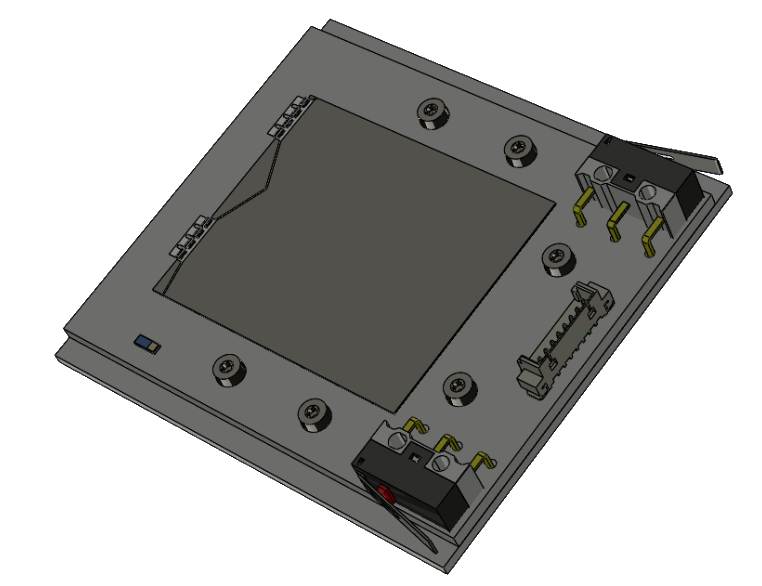
\includegraphics[width=.5\linewidth]{res/img/5_simulationanalisys/Comparisons/SLDW/BottomPCB_Solid.PNG}
      \caption{Bottom PCB in Solidworks}
      \label{fig:bottompcbsolid}
    \end{subfigure}
    \caption{Comparison between thermal and CAD model for the Bottom Board.}
    \label{fig:bottompcbim}
\end{figure}

The bulk properties of the primitive:

\begin{table}[H]
    \centering
    \resizebox{\columnwidth}{!}{
    \begin{tabular}{@{}cccccccccc@{}}
    \toprule
    \textbf{$SD\_Bottom\_Board$} & \textbf{Material} & \textbf{m (g)} & \textbf{m (kg)} & $\mathbf{m (\%)}$ & $\mathbf{V_{E} [m^3]}$ & $\mathbf{\rho [kg/m^3]}$ & $\mathbf{c_p [J/kg\cdot K]}$ & $\mathbf{k_{c.p.} [W/m\cdot K]}$ & $\mathbf{k_{i.p.} [W/m\cdot K]}$ \\ \midrule
    \textit{Bottom PCB}        & Bottom PCB            & 14.2           & 1.42E-02        & 100                 & x                      & \textbf{2133}                     & \textbf{904}                          & \textbf{0.32}                             & \textbf{170.88}                           \\
    {\ul \textit{Primitive}}         & Bottom PCB                 & 14.2           & 1.42E-02        & 100                 & 6.66E-06                 & \textbf{2133}                     & \textbf{904}                          & \textbf{0.32}                             & \textbf{170.88}                        \\ \bottomrule
    \end{tabular}
    }
    \caption{Bulk properties of the bottom PCB.}
\end{table}

The optical properties: 

\begin{table}[H]
  \centering
  \begin{tabular}{@{}cccc@{}}
    \toprule
    \textbf{Primitive} & \textbf{Material} & $\mathbf{\epsilon_{IR}}$ & $\mathbf{\alpha_{S}}$ \\ \midrule
    SD\_Bottom\_Board  & White Paint       & 0.94                     & 0.19                  \\ \bottomrule
    \end{tabular}
  \caption{Optical properties of the bottom board primitive.}
\end{table}

\subsubsection{Slider Board}
The slider board is placed directly over the bottom board. It is the support where the lateral boards rest. Its purposed
is to allow the deployment of the PocketQube by the sliding of the S/C over a rail, in the deployer. It is also a PCB,
made of two layers of copper, one of FR-4 and two of solder mask, set to white.

\paragraph{}

The most distinctive characteristic of the slider board is the fact that is presents a rectangular shaped hole in the middle
of itself. This results in a slightly more complex modeling, leading to the division of the PCB into 4 smaller primitives. The visual representation and comparison with the CAD
is presented next: 


\begin{figure}[H]
    \centering
    \begin{subfigure}{.5\textwidth}
      \centering
      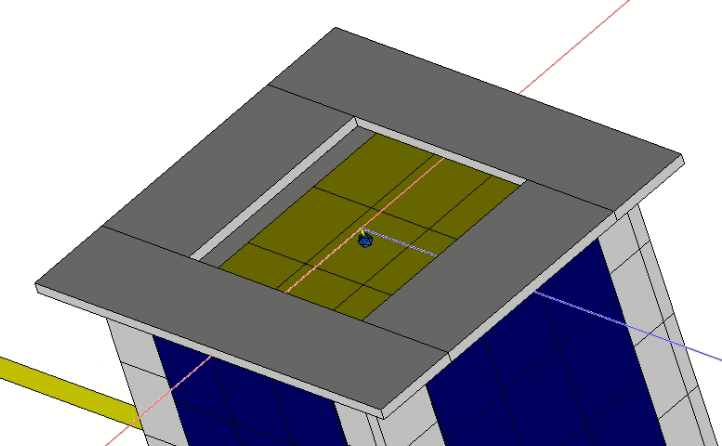
\includegraphics[width=.6\linewidth]{res/img/5_simulationanalisys/Comparisons/ESATAN/SliderPCB.PNG}
      \caption{Slider Board in ESATAN (with other components)}
      \label{fig:sliderpcb}
    \end{subfigure}%
    \begin{subfigure}{.5\textwidth}
      \centering
      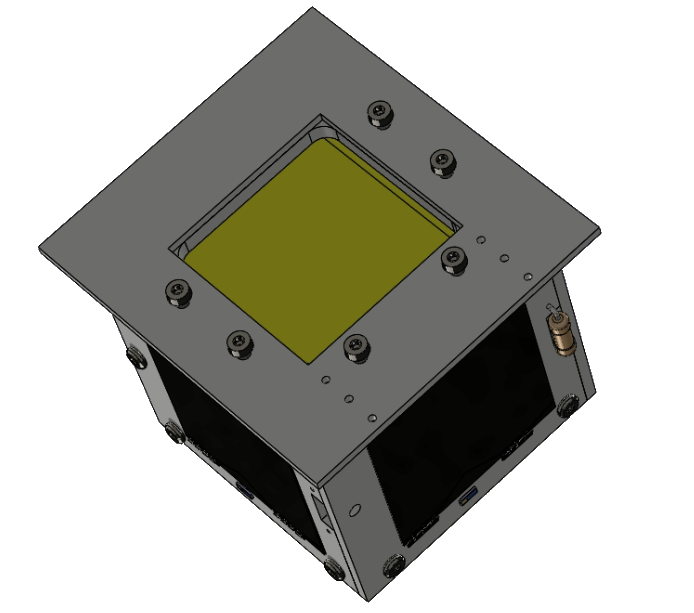
\includegraphics[width=.5\linewidth]{res/img/5_simulationanalisys/Comparisons/SLDW/SliderPCB_Solid.PNG}
      \caption{Slider Board in Solidworks (with other components)}
      \label{fig:sliderpcbsolid}
    \end{subfigure}
    \caption{Comparison between thermal and CAD model for the Slider Board (with other components)}
    \label{fig:sliderpcbim}
\end{figure}

An isolated view:

\begin{figure}[H]
    \centering
    \begin{subfigure}{.5\textwidth}
      \centering
      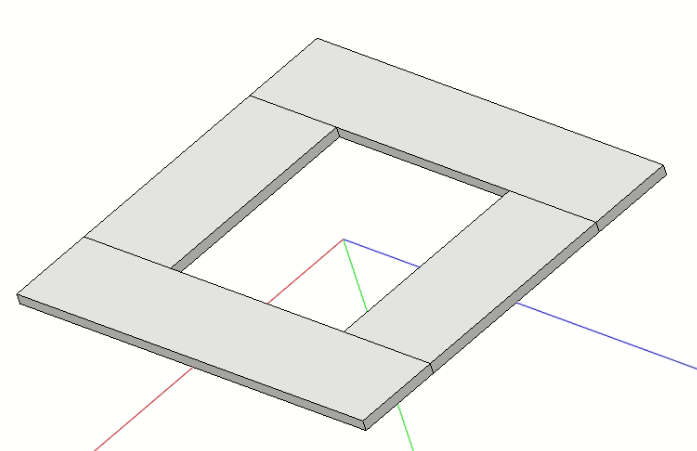
\includegraphics[width=.6\linewidth]{res/img/5_simulationanalisys/Comparisons/ESATAN/SliderPCB_raw.PNG}
      \caption{Slider Board in ESATAN (without other components).}
      \label{fig:sliderrawpcb}
    \end{subfigure}%
    \begin{subfigure}{.5\textwidth}
      \centering
      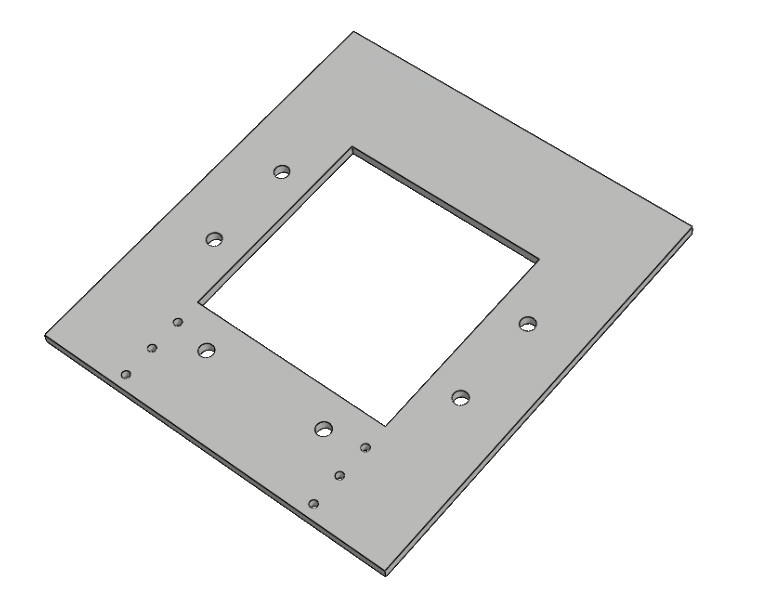
\includegraphics[width=.5\linewidth]{res/img/5_simulationanalisys/Comparisons/SLDW/SliderPCB_Raw_Solid.PNG}
      \caption{Slider Board in ESATAN (without other components).}
      \label{fig:sliderpcbrawsolid}
    \end{subfigure}
    \caption{Comparison between thermal and CAD model for the Slider Board (without other components)}
    \label{fig:sliderpcbrawim}
\end{figure}


The properties of the primitives:

\begin{table}[H]
  \centering
  \resizebox{\columnwidth}{!}{
    \begin{tabular}{@{}cccccccccc@{}}
    \toprule
    \textbf{Slider Board}                     & Material & m (g) & m (kg)   & \textbf{$\mathbf{m (\%)}$} & \textbf{$\mathbf{V_{E} [m^3]}$} & \textbf{$\mathbf{\rho [kg/m^3]}$} & \textbf{$\mathbf{c_p [J/kg\cdot K]}$} & \textbf{$\mathbf{k_{c.p.} [W/m\cdot K]}$} & \textbf{$\mathbf{k_{i.p.} [W/m\cdot K]}$} \\ \midrule
    Real Slider                               & PCB   & 8.4   & 8.40E-03 & x                          & x                               & x                                 & x                                     & x                                         & x                                         \\
    {\ul \textit{$\mathbf{SD\_Slider\_Board}$}} &          &       &          &                            &                                 &                                   &                                       &                                           &                                           \\
    SD\_Slider\_L                             & Slider   & x     & x        & \textbf{31}              & \textbf{1.33E-06}               & \textbf{1953}                     & \textbf{1050}                         & \textbf{0.30}                             & \textbf{46.76}                            \\
    SD\_Slider\_R                             & Slider   & x     & x        & \textbf{31}              & \textbf{1.33E-06}               & \textbf{1953}                     & \textbf{1050}                         & \textbf{0.30}                             & \textbf{46.76}                            \\
    SD\_Slider\_Front                         & Slider   & x     & x        & \textbf{19}              & \textbf{8.19E-07}               & \textbf{1953}                     & \textbf{1050}                         & \textbf{0.30}                             & \textbf{46.76}                            \\
    SD\_Slider\_Back                          & Slider   & x     & x        & \textbf{19}              & \textbf{8.19E-07}               & \textbf{1953}                     & \textbf{1050}                         & \textbf{0.30}                             & \textbf{46.76}                            \\
    \textit{Total}                       & Slider        & 8.4   & 8.40E-03 & \textbf{100}                 & \textbf{4.30E-06}               & \textbf{1953}                     & \textbf{1050}                         & \textbf{0.30}                             & \textbf{46.76}                            \\ \bottomrule
    \end{tabular}
  }
  \caption{Slider board primitives bulk properties. Mass percentage is calculated by volume and density.}
\end{table}

The optical properties:

\begin{table}[H]
  \centering
  \begin{tabular}{@{}cccc@{}}
  \toprule
  \textbf{Primitive} & \textbf{Material} & $\mathbf{\epsilon_{IR}}$ & $\mathbf{\alpha_{S}}$ \\ \midrule
  SD\_Slider\_Board\_X  & White Paint       & 0.94                     & 0.14                  \\ \bottomrule
  \end{tabular}
  \caption{Optical propertios of the slider board primitives.}
  \end{table}

\subsubsection{Battery and Battery Support (Case)}
The battery is a LiPo 1400mAh battery, contained within a case made of PTFE, so as to guarantee its security and minimize risk of debris is case of
a catastrophic failure. This support is also where the magnetorquer +Y PCB lies, leading to the start of the PCB stack.

\paragraph{}
The battery is simply modeled as a solid rectangular prism while,
in a similar fashion as with the slider board, the support geometry is sliced into different primitives, solid rectangular
prisms and solid cilinders on top of it.  The visual representation and comparison with the CAD
is presented next: 

\begin{figure}[H]
    \centering
    \begin{subfigure}{.5\textwidth}
      \centering
      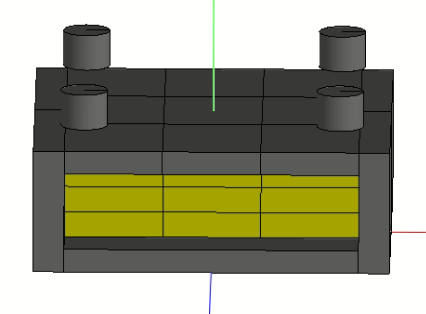
\includegraphics[width=.6\linewidth]{res/img/5_simulationanalisys/Comparisons/ESATAN/BatterySupport.PNG}
      \caption{Battery Support in ESATAN (with battery).}
      \label{fig:batterysupport}
    \end{subfigure}%
    \begin{subfigure}{.5\textwidth}
      \centering
      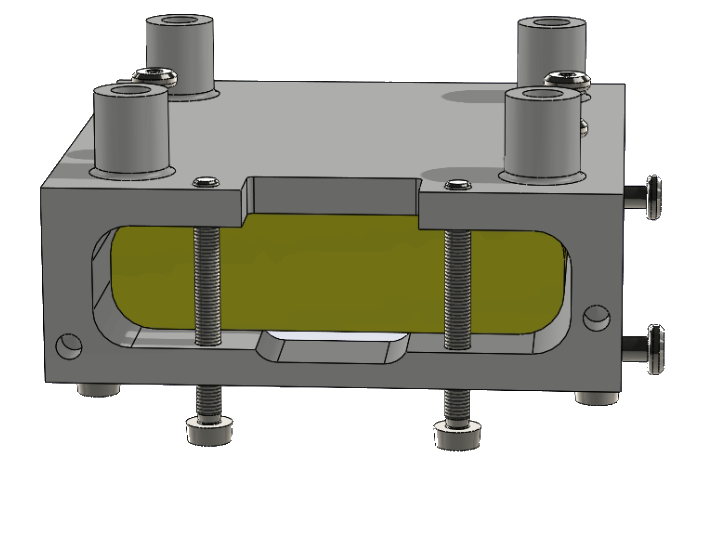
\includegraphics[width=.5\linewidth]{res/img/5_simulationanalisys/Comparisons/SLDW/BatterySupport_Solid.PNG}
      \caption{Battery Support in Solidworks (with battery).}
      \label{fig:batterysupportsolid}
    \end{subfigure}
    \caption{Comparison between thermal and CAD model for the Battery Support (with battery)}
    \label{fig:batterysupportim}
\end{figure}

An isolated view, without the battery placed inside:

\begin{figure}[H]
    \centering
    \begin{subfigure}{.5\textwidth}
      \centering
      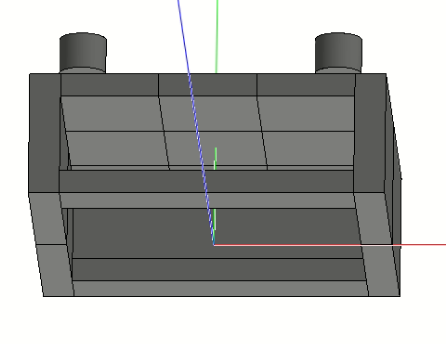
\includegraphics[width=.6\linewidth]{res/img/5_simulationanalisys/Comparisons/ESATAN/BatterySupport_raw.PNG}
      \caption{Battery Support in ESATAN (without battery).}
      \label{fig:batterysupportraw}
    \end{subfigure}%
    \begin{subfigure}{.5\textwidth}
      \centering
      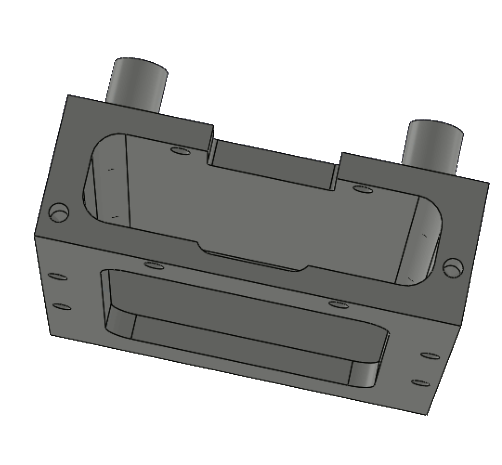
\includegraphics[width=.5\linewidth]{res/img/5_simulationanalisys/Comparisons/SLDW/BatterySupport_Raw_Solid.PNG}
      \caption{Battery Support in Solidworks (without battery).}
      \label{fig:batterysupportrawsolid}
    \end{subfigure}
    \caption{Comparison between thermal and CAD model for the Battery Support (without battery)}
    \label{fig:batterysupportrawim}
\end{figure}

The properties of the primitives:

\begin{table}[H]
  \centering
  \resizebox{\columnwidth}{!}{
  \begin{tabular}{@{}cccccccccc@{}}
  \toprule
  \textbf{SD\_Battery} & \textbf{Material} & \textbf{m (g)} & \textbf{m (kg)} & \textbf{$\mathbf{m (\%)}$} & \textbf{$\mathbf{V_{E} [m^3]}$} & \textbf{$\mathbf{\rho [kg/m^3]}$} & \textbf{$\mathbf{c_p [J/kg\cdot K]}$} & \textbf{$\mathbf{k_{c.p.} [W/m\cdot K]}$} & \textbf{$\mathbf{k_{i.p.} [W/m\cdot K]}$} \\ \midrule
  \textit{Primitive}       & LiPo Battery      & 34             & 3.40E-02        & 100                         & 1.22E-05                        & \textbf{2796}                     & \textbf{1000}                         & \textbf{0.60}                             & \textbf{2.50}                             \\ \bottomrule
  \end{tabular}
  }
  \caption{Bulk properties of the battery.}
\end{table}

\begin{table}[H]
  \centering
  \resizebox{\columnwidth}{!}{
  \begin{tabular}{@{}cccccccccc@{}}
  \toprule
  \textbf{Battery Support}                  & Material   & m (g)               & m (kg)            & \textbf{$\mathbf{m (\%)}$} & \textbf{$\mathbf{V_{E} [m^3]}$} & \textbf{$\mathbf{\rho [kg/m^3]}$} & \textbf{$\mathbf{c_p [J/kg\cdot K]}$} & \textbf{$\mathbf{k_{c.p.} [W/m\cdot K]}$} & \textbf{$\mathbf{k_{i.p.} [W/m\cdot K]}$} \\ \midrule
  \textbf{Real Support}                 & PTFE       & 30                  & 3.00E-02          & 100                          & x                               & x                                 & x                                     & x                                         & x                                         \\
  \textbf{SD\_BottStruc}                 &            &                     &                   &                            &                                 &                                   &                                       &                                           &                                           \\
  SD\_BottStruc\_BackMid                 & PTFE*      & x                   & x                 & x                          & \textbf{2.66E-06}               & \textbf{1886}                     & \textbf{1010}                         & \textbf{0.27}                            & \textbf{0.27}                            \\
  SD\_BottStruc\_DownBack                & PTFE*      & x                   & x                 & x                          & \textbf{7.98E-07}               & \textbf{1886}                     & \textbf{1010}                         & \textbf{0.27}                            & \textbf{0.27}                            \\
  SD\_BottStruc\_DownFront               & PTFE*      & x                   & x                 & x                          & \textbf{7.98E-07}               & \textbf{1886}                     & \textbf{1010}                         & \textbf{0.27}                            & \textbf{0.27}                            \\
  SD\_BottStruc\_L                       & PTFE*      & x                   & x                 & x                          & \textbf{2.94E-06}               & \textbf{1886}                     & \textbf{1010}                         & \textbf{0.27}                            & \textbf{0.27}                            \\
  SD\_BottStruc\_R                       & PTFE*      & x                   & x                 & x                          & \textbf{2.94E-06}               & \textbf{1886}                     & \textbf{1010}                         & \textbf{0.27}                            & \textbf{0.27}                            \\
  SD\_BottStruc\_Up                      & PTFE*      & x                   & x                 & x                          & \textbf{5.24E-06}               & \textbf{1886}                     & \textbf{1010}                         & \textbf{0.27}                            & \textbf{0.27}                            \\ \midrule
  \textbf{SD\_BattSuppSpacer\_1}         & PFTE** & 0.302 & 3.02E-04 & x                & \textbf{1.30E-07}               & \textbf{4207}                     & \textbf{500}                          & \textbf{15}                               & \textbf{15.00}                            \\
  Spacer                                   & PTFE       & 0.00024516          & 2.45E-07          & $<$ 1                 & x                                &  2070                              & 1010                                  & 0.27                                    & 0.27                                      \\
  Screw                                  & AlSl304SS  & 0.30175             & 3.02E-04          & $>$ 99                  & x                                &   8000                        & 500                                 & 15                                       &   15                                        \\
  {\ul Idem}                              &            &                     &                   &                            &                                 &                                   &                                       &                                           &                                           \\
  SD\_BattSuppSpacer\_2                  & PFTE**          & 0.302 & 3.02E-04 & x                 & \textbf{1.30E-07}               & \textbf{4207}                     & \textbf{500}                          & \textbf{15}                               & \textbf{15.00}                            \\
  SD\_BattSuppSpacer\_3                  & PFTE**          & 0.302 & 3.02E-04 & x                 & \textbf{1.30E-07}               & \textbf{4207}                     & \textbf{500}                          & \textbf{15}                               & \textbf{15.00}                            \\
  SD\_BattSuppSpacer\_4                  & PFTE**          & 0.302 & 3.02E-04 & x                & \textbf{1.30E-07}               & \textbf{4207}                     & \textbf{500}                          & \textbf{15}                               & \textbf{15.00}                            \\ \midrule
  \textit{Total (BottStruc)}             & PFTE(*)(**)           &   30                &  3.00E-02                 &  100                          & \textbf{1.59E-05}               & \textbf{1886}                     & \textbf{1010}                         & \textbf{0.27}                            & \textbf{0.27}                            \\ \bottomrule
  \end{tabular}
  }
  \caption{Battery support primitives bulk properties.*Adjusted density to ESATAN volume.**Considering the screw inside.}
\end{table}

The optical properties:

\begin{table}[H]
  \centering
  \begin{tabular}{@{}cccc@{}}
  \toprule
  \textbf{Primitive} & \textbf{Material} & $\mathbf{\epsilon_{IR}}$ & $\mathbf{\alpha_{S}}$ \\ \midrule
  SD\_Battery        & LiPo Battery      & 0.3                      & 0.5                   \\ \bottomrule
  \end{tabular}
  \caption{Optical propertios of the LiPo Battery.}
\end{table}

\begin{table}[H]
  \centering
  \begin{tabular}{@{}cccc@{}}
  \toprule
  \textbf{Primitive} & \textbf{Material} & $\mathbf{\epsilon_{IR}}$ & $\mathbf{\alpha_{S}}$ \\ \midrule
  SD\_BattXX\_XX     & PFTE              & 0.92                     & 0.046                 \\ \bottomrule
  \end{tabular}
  \caption{Optical properties of the battery support.}
\end{table}



\subsubsection{Vertical Conenctors}
The vertical connectors link the stack PCBs to eachother, distributing both power and data lines.
They are rectangular plastic pieces, with phosphor bronze metalic contacts that protrude out of them.

\paragraph{}

In order to model them in a simple manner, they are considered solid rectangular prisms with the average
properties of the plastic and the phosphor bronze connectors.

\paragraph{}

\begin{figure}[H]
  \centering
  \begin{subfigure}{.5\textwidth}
    \centering
    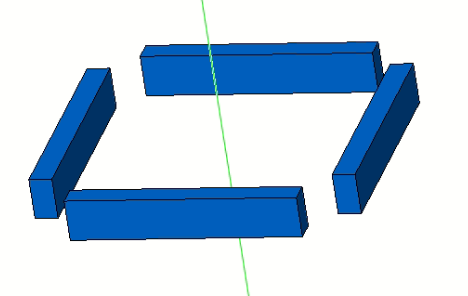
\includegraphics[width=.5\linewidth]{res/img/5_simulationanalisys/Comparisons/ESATAN/verticalconnectors.PNG}
    \caption{Set of vertical connectors in ESATAN.}
    \label{fig:verticalconnectors}
  \end{subfigure}%
  \begin{subfigure}{.5\textwidth}
    \centering
    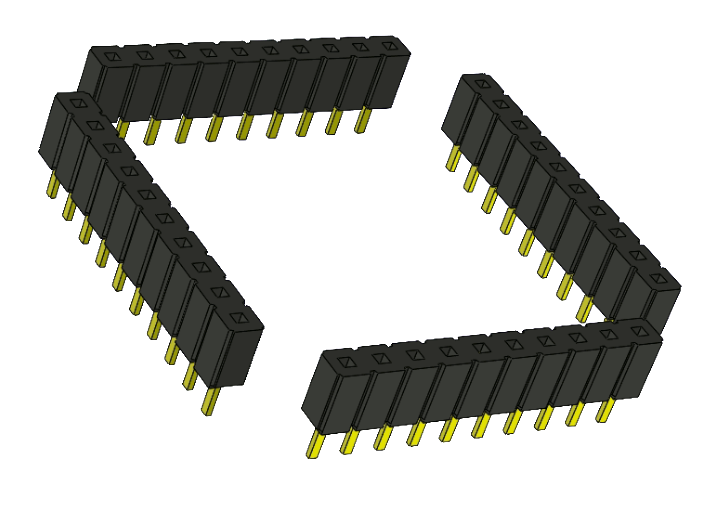
\includegraphics[width=.5\linewidth]{res/img/5_simulationanalisys/Comparisons/SLDW/verticalconectorssolid.PNG}
    \caption{Set of vertical connectors in Solidworks}
    \label{fig:verticalconectorssolid}
  \end{subfigure}
  \caption{Comparison between thermal and CAD model of the vertical connectors.}
  \label{fig:verticalconectorsim}
\end{figure}

The bulk properties assigned to them are:

\begin{table}[H]
  \centering
  \resizebox{\columnwidth}{!}{
  \begin{tabular}{@{}cccccccccc@{}}
  \toprule
  \textbf{SD\_JXSSySSz\_VC} & \textbf{Material} & \textbf{m (g)} & \textbf{m (kg)} & \textbf{$\mathbf{m (\%)}$} & \textbf{$\mathbf{V_{E} [m^3]}$} & \textbf{$\mathbf{\rho [kg/m^3]}$} & \textbf{$\mathbf{c_p [J/kg\cdot K]}$} & \textbf{$\mathbf{k_{c.p.} [W/m\cdot K]}$} & \textbf{$\mathbf{k_{i.p.} [W/m\cdot K]}$} \\ \midrule
  Inner Connector              & Phosphor Bronze   & 0.325          & 3.25E-04        & 45                       & x                               & 8800                              & 380                                   & 62.00                                     & 62.00                                     \\
  Plastic Cover                & ABS               & 0.4            & 4.00E-04        & 55                       & x                               & 1070                              & 1990                                  & 0.16                                      & 0.16                                      \\
  \textit{Primitives}               & Bulk VC (Custom)                  & 0.725          & 7.25E-04        & 100                         & 2.90E-07                        & \textbf{2502}                     & \textbf{1268}                         & \textbf{27.88}                            & \textbf{27.88}                        \\ \bottomrule
  \end{tabular}
  }
  \caption{Bulk properties of the vertical conenctors primitives.}
\end{table}

The optical properties of the vertical connectors are:

\begin{table}[H]
  \centering
  \begin{tabular}{@{}cccc@{}}
  \toprule
  \textbf{Primitive} & \textbf{Material} & $\mathbf{\epsilon_{IR}}$ & $\mathbf{\alpha_{S}}$ \\ \midrule
  SD\_JXSSySSz\_VC   & ABS               & 0.82                     & 0.94                  \\ \bottomrule
  \end{tabular}
  \caption{Optical properties of the vertical connectors.}
  \end{table}

\subsubsection{Spacers}
The spacers used are threaded by screws that run from the top PCB of the payload to the battery support.
Their purpose is to, as their name indicates, provide a specific space between the PCBs.

\paragraph{}

The actual spacers are closer to tubes than to cylinders, but are modeled as the later in order to keep the model 
simple. This does pose an issue, as the screws cannot be modeled running through them. Instead, they are 
considered when calculating the bulk properties of the volume and ignored geometrically.

The spacers are also connected by UDC in order to represent this lost conductivity provided by the screws.

\paragraph{}

Some views of the pieces and models:

\begin{figure}[H]
  \centering
  \begin{subfigure}{.5\textwidth}
    \centering
    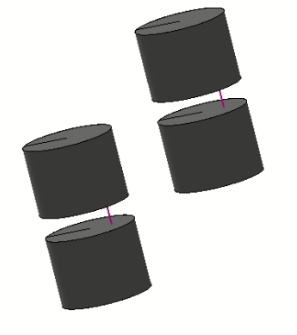
\includegraphics[width=.5\linewidth]{res/img/5_simulationanalisys/Comparisons/ESATAN/spacers.PNG}
    \caption{Set of spacers connected by UDCs.}
    \label{fig:spacersudc}
  \end{subfigure}%
  \begin{subfigure}{.5\textwidth}
    \centering
    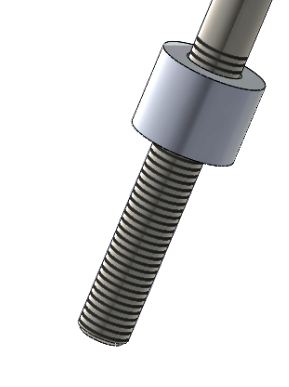
\includegraphics[width=.4\linewidth]{res/img/5_simulationanalisys/Comparisons/SLDW/spacercrossing_Solid.PNG}
    \caption{Spacer threaded by a screw.}
    \label{fig:spacersthread}
  \end{subfigure}
  \caption{Comparison of spacers in ESATAN and in Solidworks.}
  \label{fig:spacerssec5im}
\end{figure}

The bulk properties of the spacers are:

\begin{table}[H]
  \centering
  \resizebox{\columnwidth}{!}{
  \begin{tabular}{@{}cccccccccc@{}}
  \toprule
  \textbf{SD\_Spacer\_SStoSSx}             & \textbf{Material} & \textbf{m (g)} & \textbf{m (kg)} & \textbf{$\mathbf{m (\%)}$} & \textbf{$\mathbf{V_{E} [m^3]}$} & \textbf{$\mathbf{\rho [kg/m^3]}$} & \textbf{$\mathbf{c_p [J/kg\cdot K]}$} & \textbf{$\mathbf{k_{c.p.} [W/m\cdot K]}$} & \textbf{$\mathbf{k_{i.p.} [W/m\cdot K]}$} \\ \midrule
  M3x35 Hex (Partial)          & AlSl304SS         & 0.30175        & 3.02E-04        & 51                       & x                               & x                                 & 500                                   & 15                                        & 15.00                                     \\
  M3x4 Spacer (Fully)          & AlSl304SS         & 0.22           & 2.20E-04        & 37                       & x                               & x                                 & 500                                   & 15                                        & 15.00                                     \\
  M3x0.5 Spacer (Fully)        & 6063-T5           & 0.07           & 7.00E-05        & 12                       & x                               & x                      & 900                          & 209                              & 209.00                           \\
  \textit{Primitives}               & Spacer Custom                 & 0.59175        & 5.92E-04        & 1                          & 1.30E-07                        & \textbf{4552}                     & \textbf{547}                          & \textbf{15}                               & \textbf{15.00}                            \\ \bottomrule
  \end{tabular}
  }
  \caption{Bulk properties of the spacers primitives.}
\end{table}

The optical properties of the spacers:

\begin{table}[H]
  \centering
  \begin{tabular}{@{}cccc@{}}
  \toprule
  \textbf{Primitive}  & \textbf{Material} & $\mathbf{\epsilon_{IR}}$ & $\mathbf{\alpha_{S}}$ \\ \midrule
  SD\_Spacer\_SStoSSx & AlSl304SS         & 0.075                    & 0.42                  \\ \bottomrule
  \end{tabular}
  \caption{Optical properties of the spacers.}
\end{table}

\subsubsection{Magnetorquer +Y}

The +Y magnetorquer is placed on the bottom of the PCB stack, directly resting over the battery support. As is the case
with the other magnetorquers, its purpose is to provide rotation to the PQ in order to control its attitude.
\paragraph{}
Despite it having four holes in each one of its corners, in the actual spacecraft, it has been modeled as a solid rectangular
prism witout them. Some small components placed on top of the board have been ignored to simplify the model.
The visual representation and comparison with the CAD is presented next: 

\begin{figure}[H]
    \centering
    \begin{subfigure}{.5\textwidth}
      \centering
      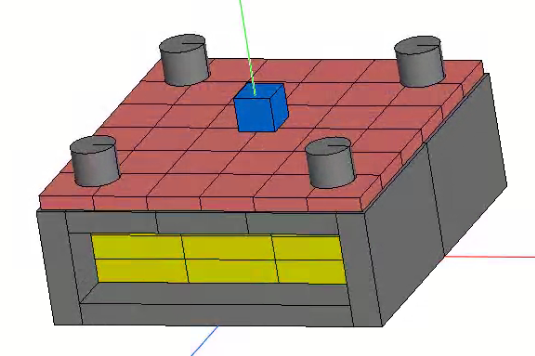
\includegraphics[width=.5\linewidth]{res/img/5_simulationanalisys/Comparisons/ESATAN/MTQ.PNG}
      \caption{MTQ +Y Model in ESATAN (Top View)}
      \label{fig:mtq}
    \end{subfigure}%
    \begin{subfigure}{.5\textwidth}
      \centering
      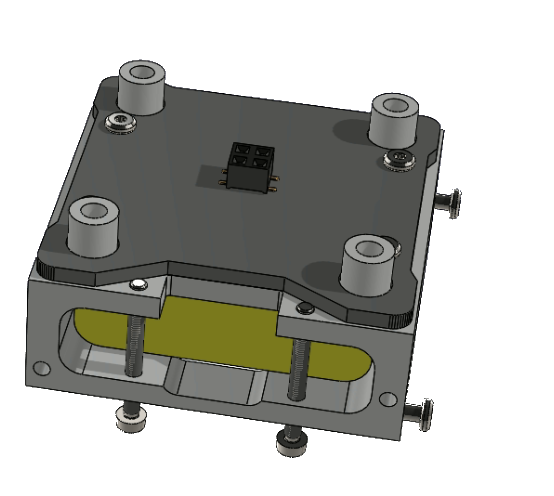
\includegraphics[width=.5\linewidth]{res/img/5_simulationanalisys/Comparisons/SLDW/MTQ_Solid.PNG}
      \caption{MTQ +Y Model in Solidworks (Top View)}
      \label{fig:mtqsolid}
    \end{subfigure}
    \caption{Comparison between thermal and CAD model for the MTG +Y (Top View)}
    \label{fig:mtqim}
\end{figure}

An isolated view:

\begin{figure}[H]
    \centering
    \begin{subfigure}{.5\textwidth}
      \centering
      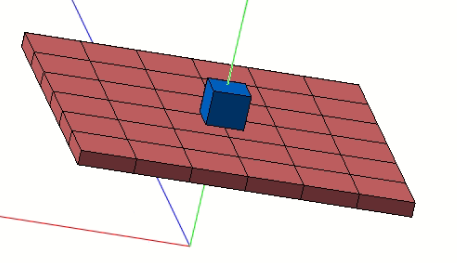
\includegraphics[width=.6\linewidth]{res/img/5_simulationanalisys/Comparisons/ESATAN/MTQ_Raw.PNG}
      \caption{MTQ +Y Model in ESATAN (Isolated View)}
      \label{fig:magraw}
    \end{subfigure}%
    \begin{subfigure}{.5\textwidth}
      \centering
      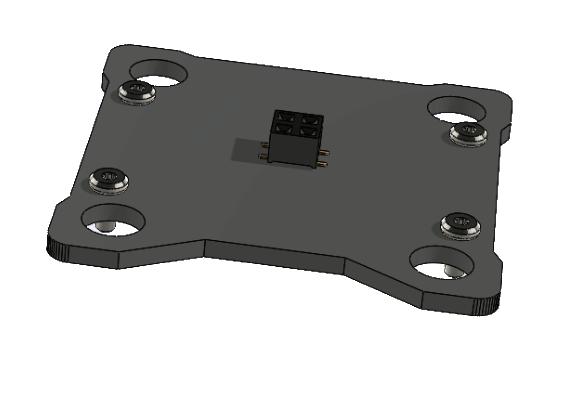
\includegraphics[width=.5\linewidth]{res/img/5_simulationanalisys/Comparisons/SLDW/MTQ_Raw_Solid.PNG}
      \caption{MTQ +Y Model in Solidworks (Isolated View)}
      \label{fig:magrawsolid}
    \end{subfigure}
    \caption{Comparison between thermal and CAD model for the MTG +Y (Isolated View)}
    \label{fig:magrawim}
\end{figure}

The bulk properties of the primitives:

\begin{table}[H]
  \centering
  \resizebox{\columnwidth}{!}{
  \begin{tabular}{@{}cccccccccc@{}}
  \toprule
  \textbf{SD\_MTQ\_PY\_Board} & \textbf{Material} & \textbf{m (g)} & \textbf{m (kg)} & \textbf{$\mathbf{m (\%)}$} & \textbf{$\mathbf{V_{E} [m^3]}$} & \textbf{$\mathbf{\rho [kg/m^3]}$} & \textbf{$\mathbf{c_p [J/kg\cdot K]}$} & \textbf{$\mathbf{k_{c.p.} [W/m\cdot K]}$} & \textbf{$\mathbf{k_{i.p.} [W/m\cdot K]}$} \\ \midrule
  MTQ PY PCB      & Y+Mag         & 6.6            & 6.60E-03        & 93                & x                               & 1630                              & 904                                   & 0.45                                      & 170.88                                    \\
  Components      & Y+Mag               & 0.5            & 5.00E-04        & 7                & x                               & 1630                              & 904                                   & 0.45                                      & 170.88                                    \\
  \textit{Total}  & Y+Mag                 & 6.6            & 6.60E-03        & 100                          & 4.05E-06                        & 1630                              & \textbf{904}                                   & \textbf{0.45}                                      & \textbf{170.88}                                   \\ \bottomrule
  \end{tabular}
  }
  \caption{Bulk properties of the magnetorquer (Positive Y axis) primitive.}
  \end{table}

  The optical properties of the MTQ+Y:

\begin{table}[H]
  \centering
  \begin{tabular}{@{}cccc@{}}
  \toprule
  \textbf{Primitive} & \textbf{Material} & $\mathbf{\epsilon_{IR}}$ & $\mathbf{\alpha_{S}}$ \\ \midrule
  SD\_MTQ\_PY\_Board & Black Coat       & 0.94                     & 0.96                  \\ \bottomrule
  \end{tabular}
  \caption{Optical properties of the MTQ+Y.}
\end{table}

\subsubsection{Attitude and Obrbit Determination and Control}

The AOCS subsystem is centralized and operated within the AOCS PCB. This PCB is placed directly over the MTQ +Y board,
held by the spacers on top of the battery support. It houses different electrical components as well as the vertical connectors
linking the subsystem with the OBC-COMMS PCB.

\paragraph{}

As will be the approach taken with the rest of the stack PCBs, the holes on the four corners have been not modeled, instead
representing the AOCS PCB by a solid rectangular prism. It is in contact with a total of eight vertical conenctors, four on each face.
It is also in contact with the PCB spacers. The ICs are modeled as Non-Geometrical Thermal Nodes, placed on top of the PCB.

\paragraph{}

The visual representation and comparison with the CAD is presented next: 


\begin{figure}[H]
    \centering
    \begin{subfigure}{.5\textwidth}
      \centering
      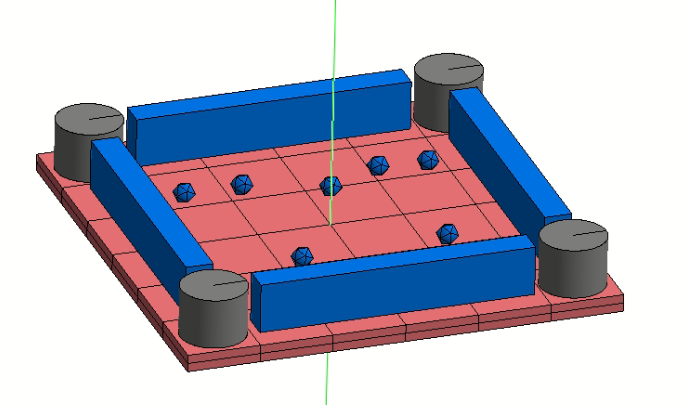
\includegraphics[width=.6\linewidth]{res/img/5_simulationanalisys/Comparisons/ESATAN/AOCS.PNG}
      \caption{AOCS Model in ESATAN (Top View)}
      \label{fig:aocs}
    \end{subfigure}%
    \begin{subfigure}{.5\textwidth}
      \centering
      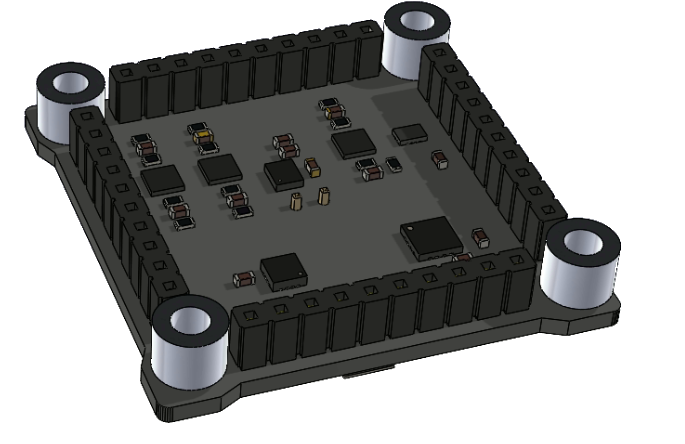
\includegraphics[width=.5\linewidth]{res/img/5_simulationanalisys/Comparisons/SLDW/AOCS_Solid.PNG}
      \caption{AOCS Model in Solidworks (Top View)}
      \label{fig:aocssolid}
    \end{subfigure}
    \caption{Comparison between thermal and CAD model for the AOCS (Top View)}
    \label{fig:aocsim}
\end{figure}

A bottom view:

\begin{figure}[H]
    \centering
    \begin{subfigure}{.5\textwidth}
      \centering
      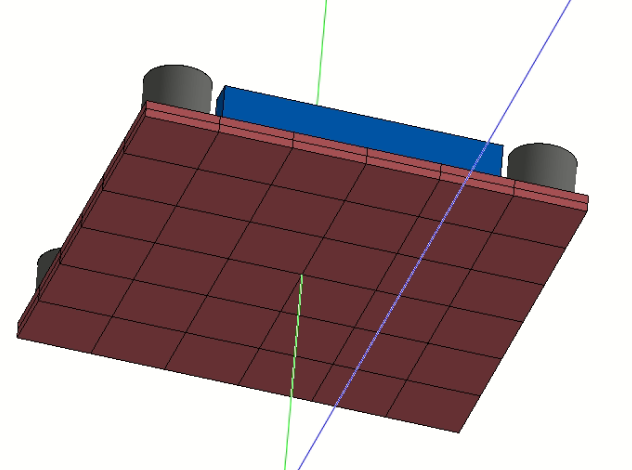
\includegraphics[width=.6\linewidth]{res/img/5_simulationanalisys/Comparisons/ESATAN/AOCS_raw.PNG}
      \caption{AOCS Model in ESATAN (Bottom View)}
      \label{fig:aocsraw}
    \end{subfigure}%
    \begin{subfigure}{.5\textwidth}
      \centering
      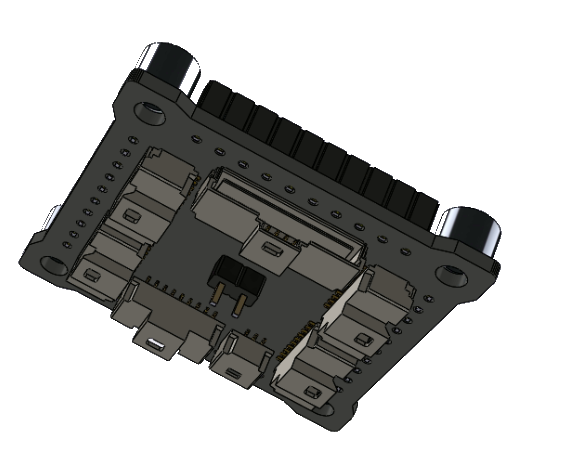
\includegraphics[width=.5\linewidth]{res/img/5_simulationanalisys/Comparisons/SLDW/AOCS_Bot_Solid.PNG}
      \caption{AOCS Model in Solidworks (Bottom View)}
      \label{fig:aocsrawsolid}
    \end{subfigure}
    \caption{Comparison between thermal and CAD model for the AOCS (Bottom View).}
    \label{fig:aocsrawim}
\end{figure}

The bulk properties of the primitive:

\begin{table}[H]
  \centering
  \resizebox{\columnwidth}{!}{
  \begin{tabular}{@{}cccccccccc@{}}
  \toprule
  \textbf{SD\_AOCS\_Board}  & \textbf{Material} & \textbf{m (g)} & \textbf{m (kg)} & \textbf{$\mathbf{m (\%)}$} & \textbf{$\mathbf{V_{E} [m^3]}$} & \textbf{$\mathbf{\rho [kg/m^3]}$} & \textbf{$\mathbf{c_p [J/kg\cdot K]}$} & \textbf{$\mathbf{k_{c.p.} [W/m\cdot K]}$} & \textbf{$\mathbf{k_{i.p.} [W/m\cdot K]}$} \\ \midrule
  AOCS PCB       & AOCS          & 5.6            & 5.60E-03        & 70                        & x                               & 3125                              & 940                                   & 0.42                                      & 91.47                                     \\
  Components     & AOCS          & 2.4            & 2.40E-03        & 30                        & x                               & 3125                              & 940                                   & 0.42                                      & 91.47                                     \\
  \textit{Primitive} & AOCS                & 8              & 8.00E-03        & 100                          & 2.56E-06                        & \textbf{3125}                     & \textbf{940}                          & \textbf{0.42}                             & \textbf{91.47}                           \\ \bottomrule
  \end{tabular}
  }
  \caption{Bulk properties of the AOCS board.}
\end{table}

\begin{table}[H]
  \centering
  \begin{tabular}{@{}cccc@{}}
  \toprule
  \textbf{Primitive} & \textbf{Material} & $\mathbf{\epsilon_{IR}}$ & $\mathbf{\alpha_{S}}$ \\ \midrule
  SD\_AOCS\_Board & Black Coat       & 0.94                     & 0.96                  \\ \bottomrule
  \end{tabular}
  \caption{Optical properties of the AOCS PCB primitive.}
\end{table}

\subsubsection{Electrical Power Supply}

The EPS is the susbsystem tasked with power gathering, distribution and management, including battery monitoring.
The PCB itself houses the MPPTs and ICs to perform the aforementioned functions. The EPS PCB is modeled as a solid rectangular
prism and the ICs as NGTN. It is in contact with a total of eight vertical conenctors, four on each face
and with the PCB spacers.

\paragraph{}

The visual representation and comparison with the CAD is presented next: 

\begin{figure}[H]
  \centering
  \begin{subfigure}{.5\textwidth}
    \centering
    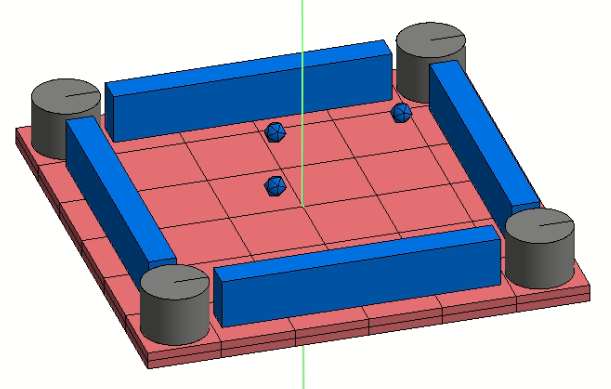
\includegraphics[width=.6\linewidth]{res/img/5_simulationanalisys/Comparisons/ESATAN/EPS.PNG}
    \caption{EPS Model in ESATAN (Top View)}
    \label{fig:eps}
  \end{subfigure}%
  \begin{subfigure}{.5\textwidth}
    \centering
    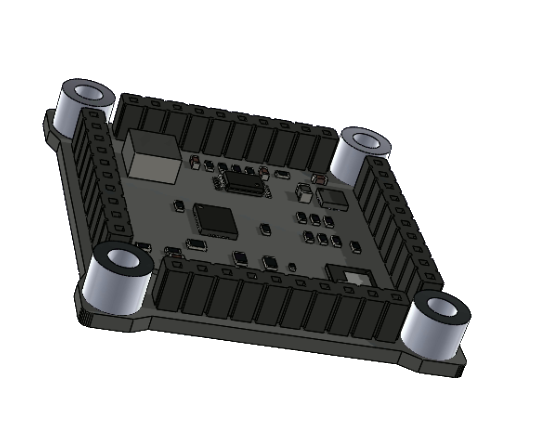
\includegraphics[width=.5\linewidth]{res/img/5_simulationanalisys/Comparisons/SLDW/EPS_Solid.PNG}
    \caption{EPS Model in Solidworks (Top View)}
    \label{fig:epssolid}
  \end{subfigure}
  \caption{Comparison between thermal and CAD model for the EPS (Top View)}
  \label{fig:epsim}
\end{figure}

A bottom view:

\begin{figure}[H]
    \centering
    \begin{subfigure}{.5\textwidth}
      \centering
      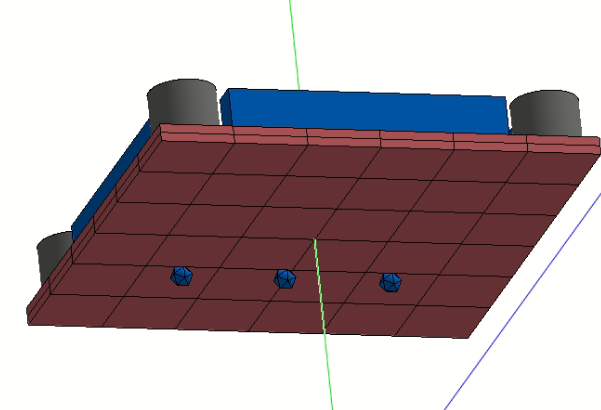
\includegraphics[width=.6\linewidth]{res/img/5_simulationanalisys/Comparisons/ESATAN/EPS_bot.PNG}
      \caption{EPS Model in ESATAN (Bottom View)}
      \label{fig:epsraw}
    \end{subfigure}%
    \begin{subfigure}{.5\textwidth}
      \centering
      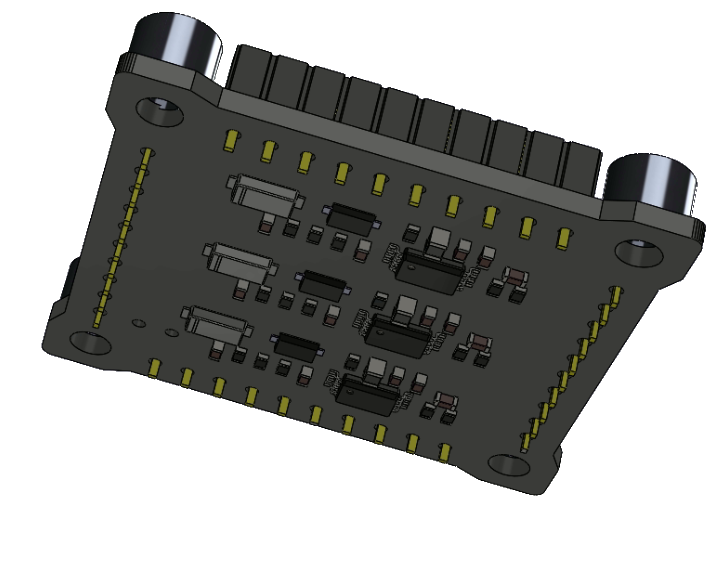
\includegraphics[width=.5\linewidth]{res/img/5_simulationanalisys/Comparisons/SLDW/EPS_bot_Solid.PNG}
      \caption{EPS Model in Solidworks (Bottom View)}
      \label{fig:epsrawsolid}
    \end{subfigure}
    \caption{Comparison between thermal and CAD model for the EPS (Bottom View).}
    \label{fig:epsrawim}
\end{figure}

The bulk properties of the EPS board:

\begin{table}[H]
  \centering
  \resizebox{\columnwidth}{!}{
  \begin{tabular}{@{}cccccccccc@{}}
  \toprule
  \textbf{SD\_EPS\_Board}  & \textbf{Material} & \textbf{m (g)} & \textbf{m (kg)} & \textbf{$\mathbf{m (\%)}$} & \textbf{$\mathbf{V_{E} [m^3]}$} & \textbf{$\mathbf{\rho [kg/m^3]}$} & \textbf{$\mathbf{c_p [J/kg\cdot K]}$} & \textbf{$\mathbf{k_{c.p.} [W/m\cdot K]}$} & \textbf{$\mathbf{k_{i.p.} [W/m\cdot K]}$} \\ \midrule
  EPS PCB        & EPS          & 5.5            & 5.50E-03        & 77                       & x                               & 2773                              & 940                                   & 0.42                                      & 91.47                                     \\
  Components     & EPS          & 1.6            & 1.60E-03        & 23                       & x                               & 2773                              & 940                                   & 0.42                                      & 91.47                                     \\
  \textit{Primitive} &     EPS              & 7.1            & 7.10E-03        & 100                          & 2.56E-06                        & \textbf{2773}                     & \textbf{940}                          & \textbf{0.42}                             & \textbf{91.47}                           \\ \bottomrule
  \end{tabular}
  }
  \caption{Bulk properties of the EPS board primitive.}
\end{table}

The optical properties of the EPS PCB primitive:

\begin{table}[H]
  \centering
  \begin{tabular}{@{}cccc@{}}
  \toprule
  \textbf{Primitive} & \textbf{Material} & $\mathbf{\epsilon_{IR}}$ & $\mathbf{\alpha_{S}}$ \\ \midrule
  SD\_EPS\_Board & Black Paint       & 0.94                     & 0.96                  \\ \bottomrule
  \end{tabular}
  \caption{Optical properties of the EPS PCB primitive.}
\end{table}

\subsubsection{On Board Computer and Communications}

The On-Board Computer and the Communications subsystems are both housed by the same PCB, at the center of the stack.
The OBC subsystem is tasked with the processing of data and management of the other subsystems. The COMMS
subsystem performs the sending and reception of RF signals containing data such as telemetry, payload data and
telecommands. 

\paragraph{}

The PCB model follows the same philosophy as the other stack PCBs and is in contact with the same number of vertical connectors and
spacers as the others. It is then modeled as a solid rectangular prisms with NGTN as ICs, including in this case, of most relevance,
the processor (STM32).

\paragraph{}

The visual representation and comparison with the CAD is presented next: 

\begin{figure}[H]
  \centering
  \begin{subfigure}{.5\textwidth}
    \centering
    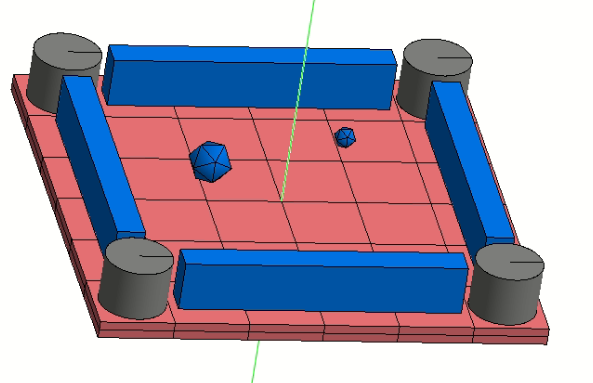
\includegraphics[width=.6\linewidth]{res/img/5_simulationanalisys/Comparisons/ESATAN/OBC.PNG}
    \caption{OBC and COMMS Model in ESATAN (Top View)}
    \label{fig:obc}
  \end{subfigure}%
  \begin{subfigure}{.5\textwidth}
    \centering
    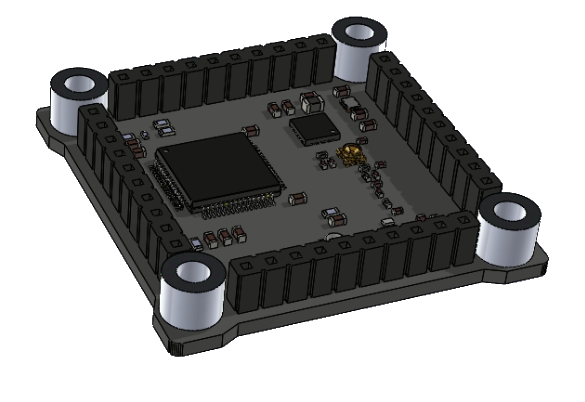
\includegraphics[width=.5\linewidth]{res/img/5_simulationanalisys/Comparisons/SLDW/OBC_Solid.PNG}
    \caption{OBC and COMMS Model in Solidworks (Top View)}
    \label{fig:obcsolid}
  \end{subfigure}
  \caption{Comparison between thermal and CAD model for the OBC and COMMS Model (Top View)}
  \label{fig:obcim}
\end{figure}

A bottom view:

\begin{figure}[H]
  \centering
  \begin{subfigure}{.5\textwidth}
    \centering
    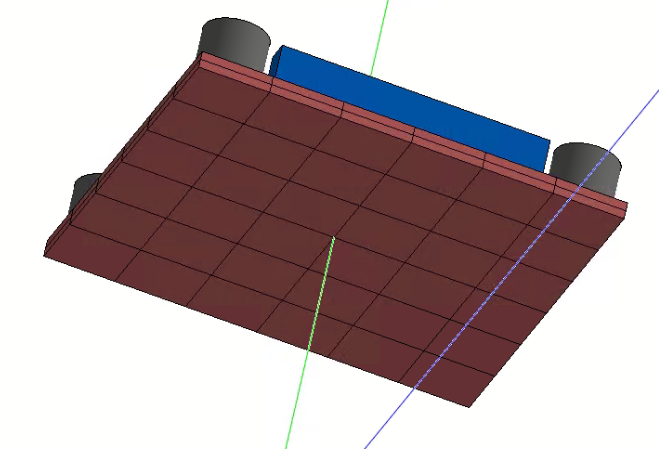
\includegraphics[width=.6\linewidth]{res/img/5_simulationanalisys/Comparisons/ESATAN/OBC_bot.PNG}
    \caption{OBC and COMMS Model in ESATAN (Bottom View)}
    \label{fig:obcbot}
  \end{subfigure}%
  \begin{subfigure}{.5\textwidth}
    \centering
    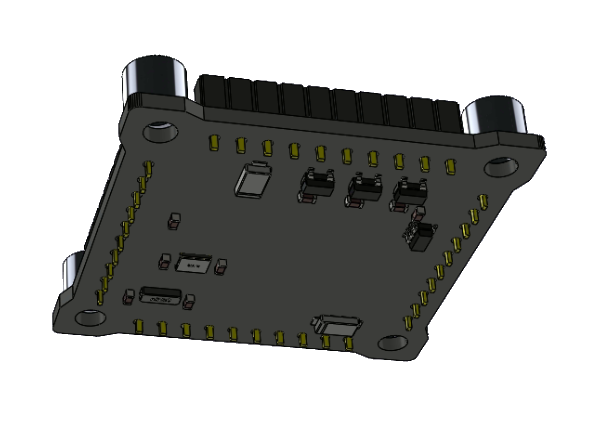
\includegraphics[width=.5\linewidth]{res/img/5_simulationanalisys/Comparisons/SLDW/OBC_Bot_Solid.PNG}
    \caption{OBC and COMMS Model in Solidworks (Bottom View)}
    \label{fig:obcbotsolid}
  \end{subfigure}
  \caption{Comparison between thermal and CAD model for the OBC and COMMS Model (Bottom View)}
  \label{fig:obcbotim}
\end{figure}

The bulk properties of the OBC primitive:

\begin{table}[H]
  \centering
  \resizebox{\columnwidth}{!}{
  \begin{tabular}{@{}cccccccccc@{}}
  \toprule
  \textbf{SD\_OBC\_Board} & \textbf{Material} & \textbf{m (g)} & \textbf{m (kg)} & \textbf{$\mathbf{m (\%)}$} & \textbf{$\mathbf{V_{E} [m^3]}$} & \textbf{$\mathbf{\rho [kg/m^3]}$} & \textbf{$\mathbf{c_p [J/kg\cdot K]}$} & \textbf{$\mathbf{k_{c.p.} [W/m\cdot K]}$} & \textbf{$\mathbf{k_{i.p.} [W/m\cdot K]}$} \\ \midrule
  OBC COMMS PCB      &  OBC COMMS         & 5.4            & 5.40E-03        & 77                       & x                               & 2734                              & 940                                   & 0.42                                      & 91.47                                     \\
  Components         &       OBC COMMS           & 1.6            & 1.60E-03        & 23                       & x                               & 2734                              & 940                                   & 0.42                                      & 91.47                                     \\
  \textit{Primitive}     &    OBC COMMS              & 7              & 7.00E-03        & 100                          & 2.56E-06                        & \textbf{2734}                     & \textbf{940}                          & \textbf{0.42}                             & \textbf{91.47}                           \\ \bottomrule
  \end{tabular}
  }
  \caption{Bulk properties of the OBC-COMMS PCB primitive.}
  \end{table}

The optical properties of the OBC\-COMMS PCB primitive:

\begin{table}[H]
  \centering
  \begin{tabular}{@{}cccc@{}}
  \toprule
  \textbf{Primitive} & \textbf{Material} & $\mathbf{\epsilon_{IR}}$ & $\mathbf{\alpha_{S}}$ \\ \midrule
  SD\_OBC\_Board & Black Coat       & 0.94                     & 0.96                  \\ \bottomrule
  \end{tabular}
  \caption{Optical properties of the OBC\-COMMS PCB primitive.}
\end{table}

\subsubsection{Payload (K-Band)}
The K-Band payload consists of two PCBs, one located directly over the OBC-COMMS PCB and the other
placed on top of an aluminum support. Over this second PCB is located a 4-patch array antenna. The objective
of the payload is to gather radiometry measurements in this band.

\paragraph{}

The modelling in this case will be split into three different main parts: the bottom PCB, the K-Band Support
and the top PCB with the antenna. The PCBs are modeled as solid rectangular prisms, with NGTNs replacing
the ICs. For the K-Band support different rectangular prisms have been combined in order to create a structure as
close to the real one as possible.

\paragraph{}

Different views of the payload and the support are provided next:

\begin{figure}[H]
  \centering
  \begin{subfigure}{.5\textwidth}
    \centering
    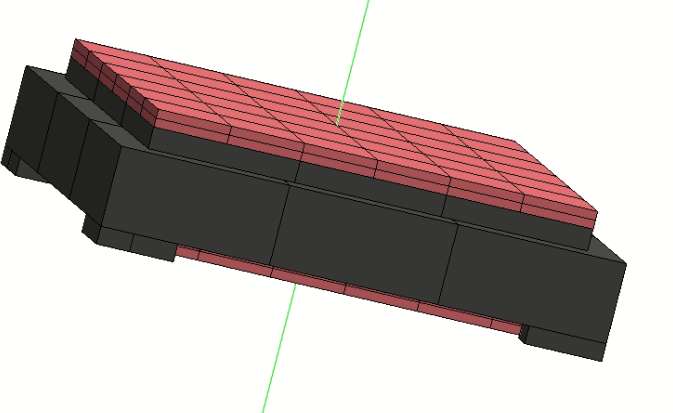
\includegraphics[width=.6\linewidth]{res/img/5_simulationanalisys/Comparisons/ESATAN/kband.PNG}
    \caption{Isolated view of the K-Band P/L in ESATAN.}
    \label{fig:kbandfull}
  \end{subfigure}%
  \begin{subfigure}{.5\textwidth}
    \centering
    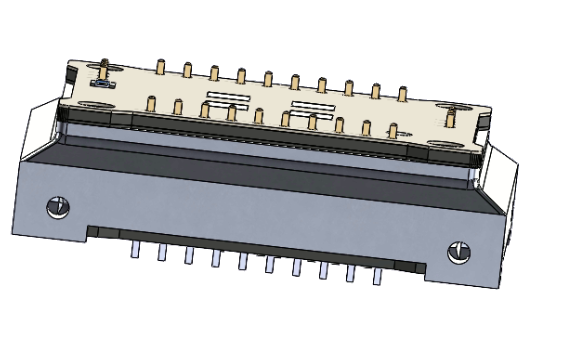
\includegraphics[width=.5\linewidth]{res/img/5_simulationanalisys/Comparisons/SLDW/kband_Solid.PNG}
    \caption{Isolated view of the K-Band P/L in Solidworks.}
    \label{fig:kbandfullsolid}
  \end{subfigure}
  \caption{Comparison between thermal and CAD model for the K-Band Payload.}
  \label{fig:kbandfullim}
\end{figure}

\begin{figure}[H]
  \centering
  \begin{subfigure}{.5\textwidth}
    \centering
    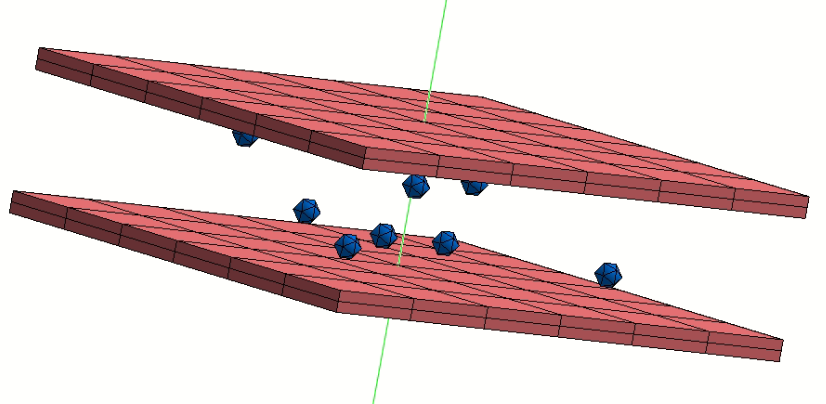
\includegraphics[width=.6\linewidth]{res/img/5_simulationanalisys/Comparisons/ESATAN/kband_raw.PNG}
    \caption{Isolated view of the K-Band P/L in ESATAN w/o support.}
    \label{fig:kbandraw}
  \end{subfigure}%
  \begin{subfigure}{.5\textwidth}
    \centering
    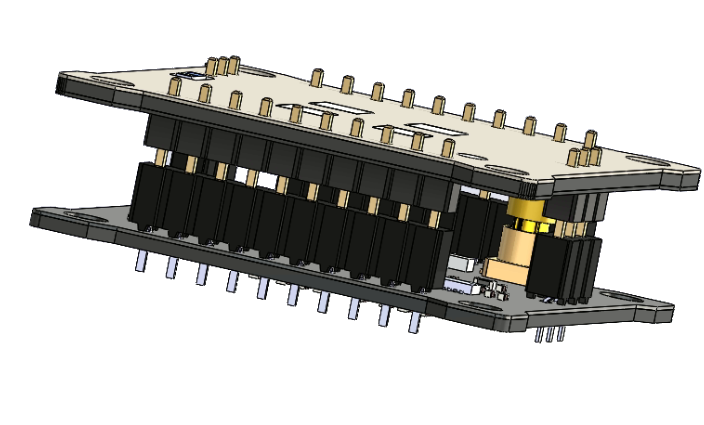
\includegraphics[width=.5\linewidth]{res/img/5_simulationanalisys/Comparisons/SLDW/kbandraw_solid.PNG}
    \caption{Isolated view of the K-Band P/L in Solidworks w/o support.}
    \label{fig:kbandrawsolid}
  \end{subfigure}
  \caption{Comparison between thermal and CAD model for the K-Band Payload without support,}
  \label{fig:kbandrawim}
\end{figure}

\begin{figure}[H]
  \centering
  \begin{subfigure}{.5\textwidth}
    \centering
    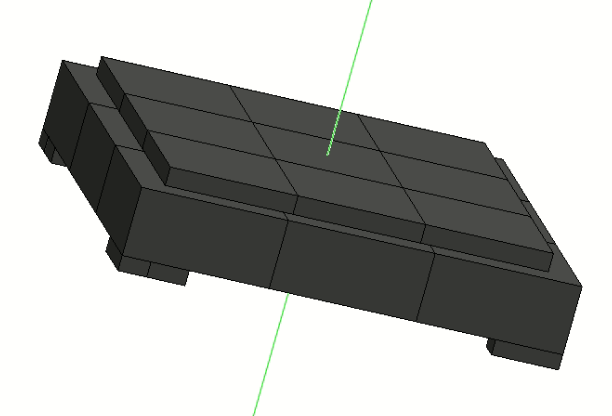
\includegraphics[width=.6\linewidth]{res/img/5_simulationanalisys/Comparisons/ESATAN/kbandsupp.PNG}
    \caption{Isolated view of the K-Band P/L support in ESATAN.}
    \label{fig:kbandsupport}
  \end{subfigure}%
  \begin{subfigure}{.5\textwidth}
    \centering
    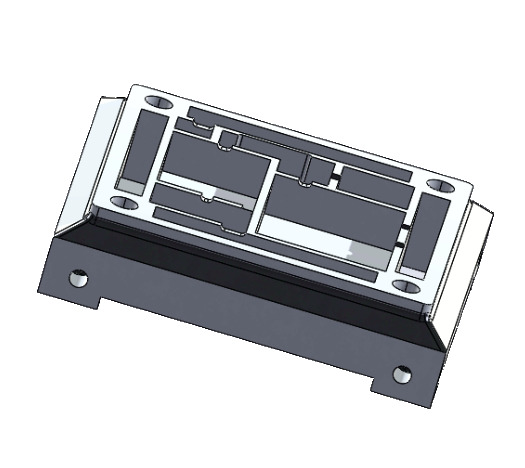
\includegraphics[width=.5\linewidth]{res/img/5_simulationanalisys/Comparisons/SLDW/kbandsupp_Solid.PNG}
    \caption{Isolated view of the K-Band P/L support in Solidworks.}
    \label{fig:kbandsupportsolid}
  \end{subfigure}
  \caption{Comparison between thermal and CAD model for the K-Band Payload support.}
  \label{fig:kbandsupportsolidim}
\end{figure}

\begin{figure}[H]
  \centering
  \begin{subfigure}{.5\textwidth}
    \centering
    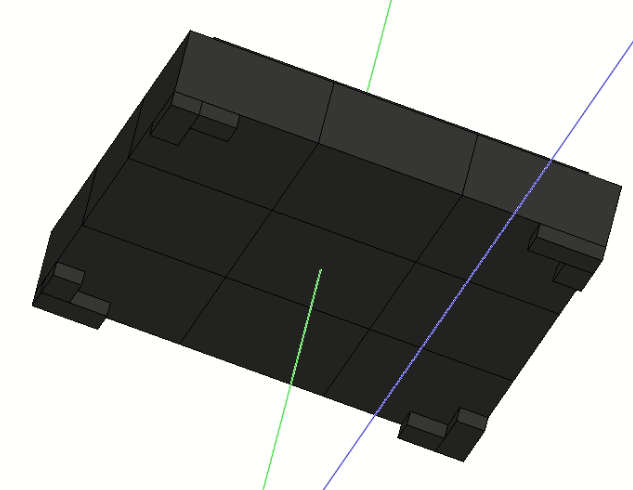
\includegraphics[width=.6\linewidth]{res/img/5_simulationanalisys/Comparisons/ESATAN/kbandsupp_Bot.PNG}
    \caption{Isolated bottom view of the K-Band P/L support in ESATAN.}
    \label{fig:kbandsupportbot}
  \end{subfigure}%
  \begin{subfigure}{.5\textwidth}
    \centering
    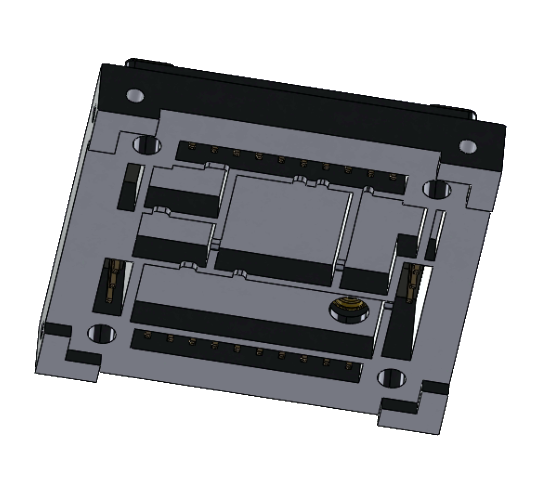
\includegraphics[width=.5\linewidth]{res/img/5_simulationanalisys/Comparisons/SLDW/kbandsuppbot_solid.PNG}
    \caption{Isolated bottom view of the K-Band P/L support in Solidworks.}
    \label{fig:kbandsupportbotsolid}
  \end{subfigure}
  \caption{Comparison between thermal and CAD model for the K-Band Payload support (bottom view).}
  \label{fig:kbandsupportsolidbotim}
\end{figure}

As it can be seen, the support has been heavily simplified, leaving the model without vertical connectors
from the top PCB to the bottom PCB. In future iterations the modeling of this conductivity might be considered.

\paragraph{}

The bulk properties of both PCBs are:

\begin{table}[H]
  \centering
  \resizebox{\columnwidth}{!}{
  \begin{tabular}{@{}cccccccccc@{}}
  \toprule
  \textbf{SD\_PL\_Board} & \textbf{Material} & \textbf{m (g)} & \textbf{m (kg)} & \textbf{$\mathbf{m (\%)}$} & \textbf{$\mathbf{V_{E} [m^3]}$} & \textbf{$\mathbf{\rho [kg/m^3]}$} & \textbf{$\mathbf{c_p [J/kg\cdot K]}$} & \textbf{$\mathbf{k_{c.p.} [W/m\cdot K]}$} & \textbf{$\mathbf{k_{i.p.} [W/m\cdot K]}$} \\ \midrule
  P/L Under PCB + Components       & KBand Under  & 9.2            & 9.20E-03        & 100                          & x                               & 3594                              & 783                                   & 0.49                                      & 110.15                                    \\
  \textit{Primitive}         &   KBand Under          & 9.2            & 9.20E-03        & 100                          & 2.56E-06                        & \textbf{3594}                     & \textbf{783}                          & \textbf{0.49}                             & \textbf{110.15}                          \\ \bottomrule
  \end{tabular}
  }
  \caption{Bulk properties of the P/L Under PCB.}
\end{table}

\begin{table}[H]
    \centering
    \resizebox{\columnwidth}{!}{
    \begin{tabular}{@{}cccccccccc@{}}
    \toprule
    \textbf{SD\_PLAntenna\_Board} & \textbf{Material} & \textbf{m (g)} & \textbf{m (kg)} & \textbf{$\mathbf{m (\%)}$} & \textbf{$\mathbf{V_{E} [m^3]}$} & \textbf{$\mathbf{\rho [kg/m^3]}$} & \textbf{$\mathbf{c_p [J/kg\cdot K]}$} & \textbf{$\mathbf{k_{c.p.} [W/m\cdot K]}$} & \textbf{$\mathbf{k_{i.p.} [W/m\cdot K]}$} \\ \midrule
    P/L Top PCB + Components      & Kband Over      & 7.6            & 7.60E-03        & 91                       & x                               & 3242                              & 905                                   & 0.29                                      & 88.53                                     \\
    Antenna          & Kband Over         & 0.7            & 7.00E-04        & 9                       & x                               & 3242                              & 905                                   & 0.29                                      & 88.53                                     \\
    \textit{Primitive}   & Kband Over                 & 8.3            & 8.30E-03        & 100                          & 2.56E-06                        & \textbf{3242}                     & \textbf{905}                          & \textbf{0.29}                             & \textbf{88.53}                            \\ \bottomrule
    \end{tabular}
    }
    \caption{Bulk properties of the P/L Top (+Antenna) PCB. The antenna properties are assumed to be the same as for the PCB (approximation).}
  \end{table}

When it comes to the K-Band support itself, the screws that run through it are considered (by the amount of volume overlapping
the defined primitive) to determine the bulk properties.

\begin{table}[H]
  \centering
  \resizebox{\columnwidth}{!}{
      \begin{tabular}{@{}cccccccccc@{}}
      \toprule
      \textbf{K-Band Support}      & \textbf{Material} & \textbf{m (g)} & \textbf{m (kg)} & \textbf{$\mathbf{m (\%)}$} & \textbf{$\mathbf{V_{E} [m^3]}$} & \textbf{$\mathbf{\rho [kg/m^3]}$} & \textbf{$\mathbf{c_p [J/kg\cdot K]}$} & \textbf{$\mathbf{k_{c.p.} [W/m\cdot K]}$} & \textbf{$\mathbf{k_{i.p.} [W/m\cdot K]}$} \\ \midrule
      Real Support                 & Alloy 7075        & 24             & 2.40E-02        & 92                       & x                               & x                                 & 960                                   & 130.00                                    & 130.00                                    \\
      Screws Crossing (0.29* 4)    & AlSl304SS         & 1.972          & 1.97E-03        & 8                      &  x                              & 8000                                 & 500                                   & 15.00                                     & 15.00                                     \\
      \textbf{SD\_PLSupp} &                   &                &                 &                            &                                 & \textbf{}                         & \textbf{}                             & \textbf{}                                 & \textbf{}                                 \\
      SD\_PLSupp\_Top              & x                 & x              & x                & x                          & 3.12E-06               & \textbf{1401}                     & \textbf{925}                          & \textbf{121.27}                           & \textbf{121.27}                           \\
      SD\_PLSupp\_Mid              & x                 & x              & x                & x                          & 1.52E-05               & \textbf{1401}                     & \textbf{925}                          & \textbf{121.27}                           & \textbf{121.27}                           \\
      SD\_PLSupp\_Aux1a            & x                 & x              & x               & x                          & 3.36E-08               & \textbf{1401}                     & \textbf{925}                          & \textbf{121.27}                           & \textbf{121.27}                           \\
      SD\_PLSupp\_Aux1b            & x                 & x              & x                & x                          & 1.92E-08               & \textbf{1401}                     & \textbf{925}                          & \textbf{121.27}                           & \textbf{121.27}                           \\
      {\ul Idem}                   &                   &                &                 &                            &                                 &                                   &                                       &                                           &                                           \\
      SD\_PLSupp\_AuxXY            & x                 & x              & x               & x                          & x                      & \textbf{1401}                     & \textbf{925}                          & \textbf{121.27}                           & \textbf{121.27}                           \\
      \textit{Total}               & KBand Support Custom            & 25.972         & 2.60E-02        & 100                          & 1.85E-05                        & \textbf{1401}                     & \textbf{925}                          & \textbf{121.27}                           & \textbf{121.27}                           \\ \bottomrule
      \end{tabular}
  }
  \caption{Bulk properties of the K-Band Support.}
\end{table}

The optical properties of these PCBs and support are:

\begin{table}[H]
  \centering
  \begin{tabular}{@{}cccc@{}}
  \toprule
  \textbf{Primitive}   & \textbf{Material}                      & $\mathbf{\epsilon_{IR}}$ & $\mathbf{\alpha_{S}}$ \\ \midrule
  SD\_PL\_Board        & Black Coat                            & 0.94                     & 0.96                  \\
  SD\_PLAntenna\_Board & Black Coat                            & 0.94                     & 0.96                  \\
  SD\_PLSupp\_XX       & \multicolumn{1}{l}{Aluminum   6063-T5} & 0.77                     & 0.80                  \\ \bottomrule
  \end{tabular}
  \caption{Optical properties of the K-Band payload.}
\end{table}

\subsubsection{Lateral Boards and Solar Panels}
The lateral boards are equipped with different sensors such as photodiodes and temperature sensors, and, most 
importatly, hold the solar panels that power the PQ. One of them also holds a thermal knife that will be used to melt
a dynnema, releasing the COMMS Antenna.

\paragraph{}

They are modeled by solid rectangular prisms. On one face of these prisms is located another rectangular prism which
represents the solar panels.

\paragraph{}

Some views to illustrate the modelling are provided next:

\begin{figure}[H]
  \centering
  \begin{subfigure}{.5\textwidth}
    \centering
    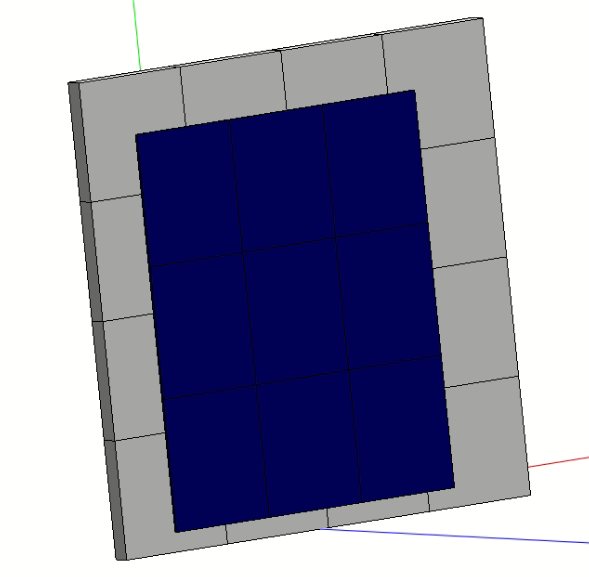
\includegraphics[width=.6\linewidth]{res/img/5_simulationanalisys/Comparisons/ESATAN/lateral.PNG}
    \caption{Lateral Board with Solar Panel in ESATAN.}
    \label{fig:lateralboard}
  \end{subfigure}%
  \begin{subfigure}{.5\textwidth}
    \centering
    \includegraphics[width=.5\linewidth]{res/img/5_simulationanalisys/Comparisons/SLDW/lateral_Solid.PNG}
    \caption{Lateral Board with Solar Panel in Solidworks.}
    \label{fig:lateralboardsolid}
  \end{subfigure}
  \caption{Comparison between thermal and CAD model for the lateral boards.}
  \label{fig:lateralboardim}
\end{figure}

\begin{figure}[H]
  \centering
  \begin{subfigure}{.5\textwidth}
    \centering
    \includegraphics[width=.6\linewidth]{res/img/5_simulationanalisys/Comparisons/ESATAN/laterals_top.PNG}
    \caption{Empty PQ view in ESATAN.}
    \label{fig:emptypq}
  \end{subfigure}%
  \begin{subfigure}{.5\textwidth}
    \centering
    \includegraphics[width=.5\linewidth]{res/img/5_simulationanalisys/Comparisons/SLDW/PQtoplat_Solid.PNG}
    \caption{Empty PQ view in Solidworks.}
    \label{fig:emptypqsolid}
  \end{subfigure}
  \caption{Comparison between thermal and CAD model of an empty PQ.}
  \label{fig:emptypqim}
\end{figure}

The bulk properties of the lateral boards and solar panels primitives:

\begin{table}[H]
  \centering
  \resizebox{\columnwidth}{!}{
  \begin{tabular}{@{}cccccccccc@{}}
  \toprule
  \textbf{SD\_PX\_Lateral\_Board}         & \textbf{Material} & \textbf{m (g)} & \textbf{m (kg)} & \textbf{$\mathbf{m (\%)}$} & \textbf{$\mathbf{V_{E} [m^3]}$} & \textbf{$\mathbf{\rho [kg/m^3]}$} & \textbf{$\mathbf{c_p [J/kg\cdot K]}$} & \textbf{$\mathbf{k_{c.p.} [W/m\cdot K]}$} & \textbf{$\mathbf{k_{i.p.} [W/m\cdot K]}$} \\ \midrule
  PX PCB                          & BotLat Bulk       & 9.8            & 9.80E-03        & 96                       & x                               & 2214                              & 904                                   & 0.45                                      & 170.88                                    \\
  Components                      & N/A               & 0.4            & 4.00E-04        & 4                       & x                               & 2214                              & 904                                   & 0.45                                      & 170.88                                    \\
  \textit{Primitive}                  & -                 & 10.2           & 1.02E-02        & 100                          & 4.61E-06                        & \textbf{2214}                     & \textbf{904}                          & \textbf{0.45}                             & \textbf{170.88}                           \\
  {\ul Idem}                      &                   &                &                 &                            &                                 &                                   &                                       &                                           &                                           \\
  \textbf{SD\_NZ\_Lateral\_Board} &                   & 10.2           & 1.02E-02        & 100                          & 4.61E-06                        & \textbf{2214}                     & \textbf{904}                          & \textbf{0.45}                             & \textbf{170.88}                           \\
  \textbf{SD\_PZ\_Lateral\_Board} &                   & 10.2           & 1.02E-02        & 100                          & 4.61E-06                        & \textbf{2214}                     & \textbf{904}                          & \textbf{0.45}                             & \textbf{170.88}                           \\  \midrule
  NX PCB                          & BotLat Bulk       & 9.8            & 9.80E-03        & 94                       & x                               & 2257                              & 904                                   & 0.45                                      & 170.88                                    \\ 
  Components(+TK)                 & N/A               & 0.6            & 6.00E-04        & 6                       & x                               & 2257                              & 904                                   & 0.45                                      & 170.88                                    \\
  \textbf{SD\_NX\_Lateral\_Board}                  & -                 & 10.4           & 1.04E-02        & 100                          & 4.61E-06                        & \textbf{2257}                              & \textbf{904}                                   & \textbf{0.45}                                      & \textbf{170.88}                                   \\ \bottomrule
  \end{tabular}
  }
  \caption{Bulk properties of the lateral boards.}
\end{table}

\begin{table}[H]
  \centering
  \resizebox{\columnwidth}{!}{
  \begin{tabular}{@{}cccccccccc@{}}
  \toprule
  \textbf{SD\_SP\_PX\_Board} & \textbf{Material} & \textbf{m (g)} & \textbf{m (kg)}   & \textbf{$\mathbf{m (\%)}$} & \textbf{$\mathbf{V_{E} [m^3]}$} & \textbf{$\mathbf{\rho [kg/m^3]}$} & \textbf{$\mathbf{c_p [J/kg\cdot K]}$} & \textbf{$\mathbf{k_{c.p.} [W/m\cdot K]}$} & \textbf{$\mathbf{k_{i.p.} [W/m\cdot K]}$} \\ \midrule
  \textbf{Total}    &   GaAs       & 0.9   & 9.00E-04 & 100                          & 3.96E-07                        & \textbf{2273}                     & \textbf{325}                          & \textbf{50}                               & \textbf{50.00}                            \\
  {\ul \textit{Idem}}        &          &       &          &                            &                                 &                                   &                                       &                                           &                                           \\
  \textbf{SD\_SP\_NX\_Board} &     GaAs     & 0.9   & 9.00E-04 & 100                          & 3.96E-07                                & \textbf{2273}                     & \textbf{325}                          & \textbf{50}                               & \textbf{50.00}                            \\
  \textbf{SD\_SP\_NY\_Board} &     GaAs     & 0.9   & 9.00E-04 & 100                          & 3.96E-07                                & \textbf{2273}                     & \textbf{325}                          & \textbf{50}                               & \textbf{50.00}                            \\
  \textbf{SD\_SP\_PZ\_Board} &     GaAs     & 0.9   & 9.00E-04 & 100                          &  3.96E-07                               & \textbf{2273}                     & \textbf{325}                          & \textbf{50}                               & \textbf{50.00}                            \\
  \textbf{SD\_SP\_NZ\_Board} &      GaAs    & 0.9   & 9.00E-04 & 100                          &  3.96E-07                               & \textbf{2273}                     & \textbf{325}                          & \textbf{50}                               & \textbf{50.00}                           \\ \bottomrule
  \end{tabular}
  }
  \caption{Bulk properties of the solar panels.}
\end{table}


The optical properties of the lateral boards and solar panels:

\begin{table}[H]
  \centering
  \begin{tabular}{@{}cccc@{}}
  \toprule
  \textbf{Primitive}             & \textbf{Material} & $\mathbf{\epsilon_{IR}}$ & $\mathbf{\alpha_{S}}$ \\ \midrule
  SD\_$\pm$X/Y/Z\_Lateral\_Board & White Paint       & 0.94                     & 0.19                  \\
  SD\_SP\_$\pm$X/Y/Z             & Gallium Arsenide  & 0.85                     & 0.91                  \\ \bottomrule
  \end{tabular}
  \caption{Optical properties of the lateral boards and the solar panels.}
\end{table}

\subsubsection{COMMS Antenna}
The COMMS Antenna is a $\lambda/4$ monopole tuned to a frequency of 868MHz. It transmits and recevies RF signals
to and from the ground station. It is soldered and screwed into a lateral board, which in turn is connected to the 
COMMS PCB.

\paragraph{}

The COMMS Antenna is modeled as a solid rectangular prism connected with a UDC to a lateral board.

\begin{figure}[H]
  \centering
  \begin{subfigure}{.5\textwidth}
    \centering
    \includegraphics[width=.5\linewidth]{res/img/5_simulationanalisys/Comparisons/ESATAN/commsantenna.PNG}
    \caption{COMMS Antenna model in ESATAN.}
    \label{fig:commsantenna}
  \end{subfigure}%
  \begin{subfigure}{.5\textwidth}
    \centering
    \includegraphics[width=.5\linewidth]{res/img/5_simulationanalisys/Comparisons/SLDW/commsantenna.png}
    \caption{PoCat-1 image.}
    \label{fig:commsantennasolid}
  \end{subfigure}
  \caption{Comparison between thermal model and image of the COMMS Antenna.}
  \label{fig:commsantennaim}
\end{figure}

The bulk properties of the antenna are:

\begin{table}[H]
  \centering
  \resizebox{\columnwidth}{!}{
    \begin{tabular}{@{}cccccccccc@{}}
      \toprule
      \textbf{SD\_COMMS\_Antenna} & \textbf{Material} & \textbf{m (g)} & \textbf{m (kg)} & \textbf{$\mathbf{m (\%)}$} & \textbf{$\mathbf{V_{E} [m^3]}$} & \textbf{$\mathbf{\rho [kg/m^3]}$} & \textbf{$\mathbf{c_p [J/kg\cdot K]}$} & \textbf{$\mathbf{k_{c.p.} [W/m\cdot K]}$} & \textbf{$\mathbf{k_{i.p.} [W/m\cdot K]}$} \\ \midrule
      \textit{Primitive}              & AlSl304SS         & 5.7            & 5.70E-03        & 100                          & 7.13E-07                        & \textbf{8000}                       & \textbf{500}                          & \textbf{15}                               & \textbf{15}                            \\ \bottomrule
      \end{tabular}
  }
  \caption{Bulk properties of the COMMS Antenna.}
\end{table}

And the optical properties:
\begin{table}[H]
  \centering
  \begin{tabular}{@{}cccc@{}}
  \toprule
  \textbf{Primitive} & \textbf{Material} & $\mathbf{\epsilon_{IR}}$ & $\mathbf{\alpha_{S}}$ \\ \midrule
  SD\_COMMS\_Antenna & AlSl304SS         & 0.075                    & 0.42                  \\ \bottomrule
  \end{tabular}
  \caption{Optical properties of the COMMS antenna.}
  \end{table}